\documentclass[a4paper]{report}

\usepackage{../mathstemplate}

\date{III семестр, осень 2023 г.}
\title{Дифференциальные уравнения и динамические системы. Неофициальный конспект}
\author{Лектор: Сергей Юрьевич Пилюгин  \\ Конспектировал Леонид Данилевич}
% sergeipil47@mail.ru
% receive at (mathbsc2022|ds_2022)

\begin{document}
    \shorthandoff{"}
    \maketitle
    \tableofcontents
    \newpage
    \setcounter{lection}{0}


    \section*{Литература}
    \numbers{
        \item Юрий Николаевич Бибиков, <<Общий курс обыкновенных дифференциальных уравнений>>
        \item Владимир Игоревич Арнольд, <<Обыкновенные дифференциальные уравнения>>
        \item Сергей Юрьевич Пилюгин, <<Пространства динамических систем>>
    }


    \chapter{Интегрирование уравнений первого порядка}
    \newlection{1 сентября 2023 г.}
    Обыкновенное дифференциальное уравнение --- уравнение, в которой независимая переменная (в обыкновенных --- скалярная) обычно обозначается $x$,
    а искомая функция --- $y(x)$.

    Дифференциальное уравнение порядка $m$ --- уравнение вида $f\left(x, y, y', \dots, y^{(m)}\right) = 0$.

    Основателем теории дифференциальных уравнений (и современного анализа вообще) считается Исаак Ньютон.
    Важным примером дифференциального уравнения можно считать уравнение движения материальной точки по прямой --- сила, действующая на точку как-то зависит от времени, координаты точки, и её скорости, получается уравнение $m \ddot{x} = f(t, x, \dot{x})$.


    Ищем функцию $y(x)$ из уравнения $y' = f(x, y)$.

    В данном курсе всегда будем предполагать, что функция $f$ (\emph{правая часть дифференциального уравнения}) непрерывна.

    Пусть $G \subset \R^2_{x,y}$ --- \emph{область} (открытое связное множество), причём $f \in C(G)$, то есть $f$ непрерывна в данной области.

    Функция $y: (a, b) \map \R$ называется решением уравнения $y' = f(x, y)$ на промежутке $(a, b)$, если
    \numbers{
        \item $y$ дифференцируема.
        \item $\defset{(x, y(x))}{x \in (a, b)} \subset G$.
        \item Выполняется равенство $y'(x) \equiv f(x, y(x))$ при $x \in (a, b)$.
    }
    \note{
        Две функции, заданные на разных промежутках --- разные решения.
    }
    \examples{
        \item $y' = ky$, где $k \in \R$. В качестве $G$ естественно брать всю плоскость $\R^2_{x,y}$.
        Из анализа известно, что любая функция $y(x) = C \cdot e^{kx}$ является решением на любом промежутке.
        \note{В данном случае ни $C = 0$, ни $k = 0$ не являются проблемой.}
        \definition[Интегральная кривая]{График произвольного решения.}
        Если область --- существования и единственности, то интегральные кривые данного уравнения покрывают её всю: через каждую точку проходит ровно одна из кривых.
        \[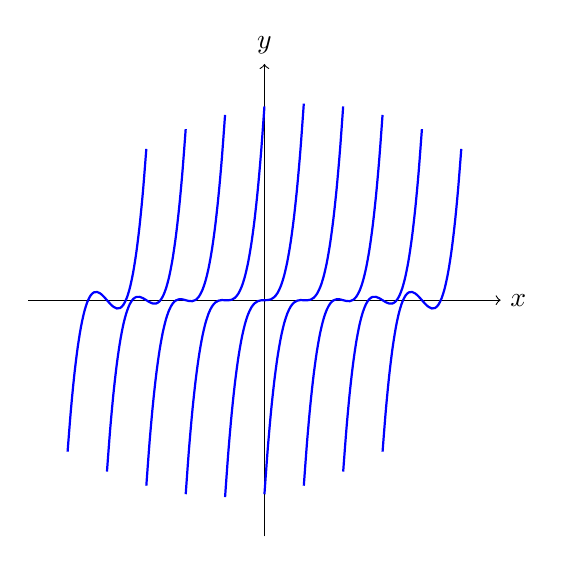
\begin{tikzpicture}
            \draw[->] (-3,0) -- (3,0) node[right] {$x$};
            \draw[->] (0,-3) -- (0,3) node[above] {$y$};
            \foreach \c in {-2,-1.5,...,2} {
                \draw[scale=1,domain={-0.5}:{0.5},smooth,variable=\x,blue,line width=0.8pt] plot ({\x-\c},{20 * (\x - 0.12 * \c) * \x * (\x + 0.12 * \c)});
            }
        \end{tikzpicture}\]
        \item Рассмотрим уравнение $y' = \frac{1}{2y}$. Функция не определена при $y = 0$, естественно возникают две области $G_1 = \defset{(x, y)}{y > 0}$ и $G_2 = \defset{(x, y)}{y < 0}$.
        На каждой из них функция определена и непрерывна.

        \[y'(x) = \frac{1}{2y(x)} \quad \then \quad 2y(x)y'(x) = 1 \quad \then \quad (y^2(x))' = 1\]
        Теперь уже из анализа понятно, что $y^2(x)$ имеет вид $x + C$ для некой константы $C$.

        В $G_1$ решением является $y(x) = \sqrt{x + C}$, в $G_2$ --- $y(x) = -\sqrt{x + C}$. Эти решения определены не для всех значений $x$, а только для тех, где $x + C > 0$ (равенство нулю также недопустимо, необходимо существование производной).
    }
    Обычно у дифференциального уравнения бесконечно много решений, даже не принимая в расчёт, что они могут быть заданы на разных промежутках.

    Естественно искать решения с некоторыми свойствами --- ограниченные решения, периодические решения, так далее.

    Основное время мы посвятим так называемой \textbf{задаче Коши}.
    В неё фиксирована точка $(x_0, y_0) \in G$, а функция $y: (a, b) \map \R$ называется \emph{решением задачи Коши с начальными данными $(x_0, y_0)$}, если $y$ --- решение на $(a, b)$, причём $x_0 \in (a, b), y(x_0) = y_0$.
    Геометрический смысл задачи Коши --- решение с интегральной кривой, проходящей через $(x_0, y_0)$.

    В вопросе о единственности решения Коши простое определение дать непросто --- всякое решение на каком-то интервале можно сузить на меньший интервал, и никакое решение абсолютно единственным являться не может.

    \definition[Точка единственности решения задачи Коши]{
        Точка $(x_0, y_0) \in G$, такая, что для любых двух решений $y_1(x), y_2(x)$ задачи Коши с начальными данными $(x_0, y_0)$ существует интервал $(\alpha, \beta) \ni x_0$, такой, что $y_1(x) \equiv y_2(x)$ при $x \in (\alpha, \beta)$.
    }
    \counterexample{
        \item Рассмотрим уравнение $y' = 3 \sqrt[3]{y^2}$.
        Здесь правая часть определена и непрерывна на всей плоскости.

        Рассмотрим задачу Коши с начальными данными $(0, 0)$.

        Есть очевидное решение $y'(x) \equiv 0, x \in \R$.

        Есть решение $y(x) = \all{0,& x < 0 \\x^3,&x > 0}$.
        Это тоже решение, так как функция дифференцируема всюду (в том числе в нуле), причём равенство выполняется.

        Эти два решения не совпадают ни на каком интервале, содержащем $0$, таким образом $(0,0)$ точкой единственности данной задачи Коши не является.

        Тем не менее, вскоре мы увидим, что, например, точка $(1, 1)$ --- точка единственности соответствующей задачи Коши.
    }
    \theorem[Теорема существования]{
        Если правая часть непрерывна в данной области $G$, то для любой точки $(x_0, y_0) \in G$ существует решение задачи Коши.
        \provehere{
            Теорема Пеано с существовании решения:~(\cref{peano}).
        }
    }
    \theorem[Теорема единственности]{
        Если и $f$, и $\der{f}{y}$ обе непрерывны в данной области $G$, любая точка $(x_0, y_0) \in G$ --- точка единственности.
        \provehere{
            Любая из теорем существования и единственности:~(\cref{picard}) или (\cref{compressing}).
        }
    }
    Если выполнены оба условия, то $G$ --- область существования и единственности.

    Рассмотрим уравнение $y' = f(x, y)$ на $G$.
    Рассмотрим точку $(x_0, y_0)$, и проведём через эту точку соответствующую интегральную кривую.
    В точке $(x_0, y_0)$ к ней можно провести касательную, её угловой коэффициент будет $y'(x_0) = f(x_0, y_0)$.
    \definition[Поле направлений]{
        Проведём через каждую точку $(x_0, y_0)$ отрезок с угловым коэффициентом $f(x_0, y_0)$.
    }
    \fact{
        $y(x)$ --- решение на промежутке $(a, b)$ $\iff \forall x \in (a, b): y(x)$ касается отрезка из поля направлений (соответствующего точке $(x, y(x))$).
    }

    Вопрос о решении уравнений достаточно сложный, сейчас мы будем рассматривать несколько типов уравнений, для которых решения можно находить <<в более или менее явном виде>>.


    \section{Уравнения первого порядка, разрешённые относительно частных производных}
    Рассмотрим уравнение $y' = f(x, y), f \in C(G)$.

    Функция $u: H \map \R$, где область $H \subset G$, называется \emph{(первым) интегралом} уравнения в $H$, если
    \numbers{
        \item $u \in C^1(H)$.
        \item $\der{u}{y} \ne 0$ в $H$.
        \item Для любого решения $y(x)$ на $(a, b)$, такого, что $\forall x \in (a, b): (x, y(x)) \in H$ функция $u(x, y(x))$ является постоянной на $x \in (a, b)$.
    }

    Вспомним точную формулировку теоремы о неявной функции.
    \theorem[О неявной функции]{
        Рассмотрим функцию $F: H \map \R$, где $H \subset \R^2$, такую, что $F \in C^1(H)$, $\exists (x_0, y_0) \in H: F(x_0, y_0) = 0$, причём $\der{F}{y}(x_0, y_0) \ne 0$.

        Тогда существуют два интервала $I, J \subset \R$ ($I \ni x_0, J \ni y_0$), и существует функция $z \in C^1(I)$, такая, что
        \[F(x, y) = 0, x \in I, y \in J \iff y = z(x)\]
    }
    \theorem[Об интеграле]{
        Пусть $u(x, y)$ --- интеграл в $H \subset G$. Тогда $\forall (x_0, y_0) \in H$ найдутся интервалы $I \ni x_0, J \ni y_0$, и $\exists Y \in C^1(I)$, такие что
        \numbers{
            \item $Y$ --- решение задачи Коши с начальными данными $(x_0, y_0)$
            \item $\forall (x, y) \in I \times J: u(x, y) = u(x_0, y_0) \iff y = Y(x)$.
        }
        \provehere{
            Рассмотрим $F(x, y) \coloneqq u(x, y) - u(x_0, y_0)$.
            Функция $F$ удовлетворяет условиям теоремы о неявной функции ($\der{F}{y} \ne 0$ по определению \emph{интеграла}).

            По теореме о неявной функции $\exists z(x)$, такая, что $F(\cdot, \cdot)$ на множестве $I \times J$ обнуляется ровно на точках вида $(x, z(x))$.

            С другой стороны, по теореме существования найдётся решение $y(x)$ на промежутке $I_0 \ni x_0$. Можно сузить $I_0$ так, чтобы $I_0 \subset I, y(I_0) \subset J$.
            По определению интеграла $u(x, y(x))$ постоянно, то есть равно $u(x_0, y(x_0))$.

            Отсюда видим, что сужение $z$ на $I_0\times J_0$ и является искомой функцией $Y$ --- неким сужением $y$.
        }
    }
    \newlection{8 сентября 2023 г.}
    \[y' = f(x), f \in C(a, b)\]
    Из анализа известно, что для любой точки $(x_0, y_0) \in (a, b) \times \R$ существует и единственно решение, проходящее через данную точку
    \[y(x) = y_0 + \int\limits_{x_0}^{x}f(t)\d t\]


    \section{Дифференциальные уравнения с разделяющимися переменными}
    \[y' = m(x)n(y)\]
    где $m \in C(a, b), n \in C(\alpha, \beta)$.

    Имеет смысл искать решение в области $G = (a, b) \times (\alpha, \beta)$.

    Предположим, что $\exists y_0 \in (\alpha, \beta): n(y_0) = 0$.
    Тогда в числе прочих решений есть $y(x) \equiv y_0$, определённая при $x \in (a, b)$.

    Теперь что происходит в прочих местах?
    Пусть $I = (\alpha', \beta')$ выбрано так, что $\forall y \in I: n(y) \ne 0$.
    Обозначим $I_0 = (a, b)$.
    Выберем $x_0 \in I_0, y_0 \in I$.

    При подстановке $y'(x) = m(x)n(y(x))$ получаем уравнение $\frac{y'(x)}{n(y(x))} = m(x)$, что можно проинтегрировать.
    \gather{
        \int\limits_{x_0}^{x}\frac{y'(t)}{n(y(t))}\d t = \int\limits_{x_0}^{x}m(s)\d s\\
        \Big\|y(t) = z \qquad y'(t)\d t = \d z\Big\| \\
        \int\limits_{y(x_0)}^{y(x)}\frac{\d z}{n(z)} = \int\limits_{x_0}^{x}m(s)\d s
    }
    Введём две первообразные $M(x) = \int\limits m(x)\d x$ (определена на $(a, b)$) и $N(y) = \int\limits \frac{\d y}{n(y)}$ (определена на $I$).

    Тогда мы получаем равенство $N(y(x)) - M(x) = N(y(x_0)) - M(x_0)$.
    Отсюда мы получаем \emph{интеграл} $U(x, y) = N(y) - M(x)$.
    В самом деле,
    \bullets{
        \item $U \in C^1((a, b) \times (\alpha', \beta'))$.
        \item $\der{U}{y} = \frac{1}{n(y)} \ne 0$.
        \item Для всякого решения $y(x)$
        \[\frac{\d}{\d x}U(x, y(x)) = \der{}{x}U(x, y(x)) + \der{}{y}U(x, y(x)) \cdot y'(x) = -m(x) + \frac{1}{n(y(x))}m(x)n(y(x)) = 0\]
    }


    \section{Замена переменных}
    В уравнении $y' = f(x, y)$ можно ввести новую независимую переменную $v$, и новую искомую функцию $w$, связанные тождествами
    \[x = V(v, w) \quad y = W(v, w)\]
    Подставив, мы получим новое дифференциальное уравнение, которое может быть легче решить.
    \examples{
        \item $y' = f(ax + by)$. Будем считать, что $ab \ne 0$, иначе неинтересно.
        Оставив $x$ независимой переменной, заменим $w = ax + by$.
        Теперь $w' = a + b y' = a + b f(w)$, что есть уравнение с разделяющимися переменными.
        \item Ещё одним примером является уже знакомое нам уравнение с разделяющимися переменными $y' = m(x)n(y)$ при $n(y(x)) \ne 0$.

        Тут, заменив, $w = \int\limits \frac{1}{n(y)}\d y = N(y)$ получаем уравнение $\frac{\d w}{\d x} = \frac{1}{n(y)}\cdot y' = m(x)$.
    }


    \section{Линейное дифференциальное уравнение первого порядка}
    \[y' = p(x)y + q(x)\]
    где $p, q \in C(a, b)$.
    Обозначив $f(x, y) = p(x)y + q(x)$ на области $G = (a, b) \times \R$, видим, что $f, \der{f}{y} \in C(G)$, откуда $G$ --- область существования и единственности.

    \numbers{
        \item Рассмотрим \emph{однородное уравнение} $y'(x) = p(x)y$, как бы заменив $q(x)$ на $0$.

        \bullets{
            \item $y(x) \equiv 0$ --- решение на $x \in (a, b)$.
            \item Рассмотрим $G_+ = \defset{(x, y)}{x \in (a, b), y > 0}$.
            Пусть $(x_0, y_0) \in G_+$.
            \gather{
                \int\limits_{x_0}^{x}\frac{\d y}{y(t)} = \int\limits_{x_0}^{x}p(s)\d s\\
                \log(y(x)) - \log(y(x_0)) = \int\limits_{x_0}^{x}p(s)\d s \\
                y(x) = y_0 \cdot \exp\left(\int\limits_{x_0}^{x}p(s)\d s\right)\\
            }
            Это решение, проходящее через точку $(x_0, y_0)$.
            \item Для области $G_-$ аналогичные рассуждения выдают тот же ответ $y(x) = y_0 \cdot \exp\left(\int\limits_{x_0}^{x}p(s)\d s\right)$.
        }
        Таким образом, множество всех решений --- это $\defset{y(x) = y_0 \cdot \exp\left(\int\limits_{x_0}^{x}p(s)\d s\right)}{(x_0, y_0) \in G}$, причём здесь записано единственное решение, проходящее через $(x_0, y_0)$.
        Тем не менее, пока то, что $G$ --- область существования и единственности даёт гарантии лишь локальной единственности, и то, что никаких других решений нет (кроме сужений данного), мы докажем позднее~(\cref{common_theorem}).
        \item \textbf{Метод Лагранжа (метод вариации произвольной постоянной)}.
        Будем искать решения неоднородного уравнения $y' = p(x)y + q(x)$ в виде $y(x) = c(x)\exp\left(\int\limits_{x_0}^{x}p(s)\d s\right)$, где $c \in C^1(a, b)$.

        Продифференцировав, получим $y'(x) = c'(x)\exp\left(\int\limits_{x_0}^{x}p(s)\d s\right) + c(x)p(x)\exp\left(\int\limits_{x_0}^{x}p(s)\d s\right)$.

        Хочется, чтобы выполнялось равенство $y'(x) = p(x)y + q(x)$, это эквивалентно равенству $c'(x)\exp\left(\int\limits_{x_0}^{x}p(s)\d s\right) = q(x)$, откуда получаем
        \[c(x) = \int q(x)\exp\left(-\int\limits_{x_0}^{x}p(s)\d s\right)\d x\]

        \item Заметим, что если $y_1(x)$ --- решение неоднородного уравнения ($y'(x) = p(x)y + q(x)$), $y_2(x)$ --- решение соответствующего однородного ($y'(x) = p(x)y$), то $y_1 + y_2$ --- тоже решение данного неоднородного уранвения.

        Получаем довольно громоздкую формулу для решения задачи Коши
        \[y(x) = \exp\left(\int\limits_{x_0}^{x}p(t)\d t\right)\cdot \left(y_0 + \int\limits_{x_0}^{x}q(t)\exp\left(\int\limits_{x_0}^{x}p(s)\d s\right)\d t\right)\]
    }


    \section{Уравнение Бернулли}
    \[y' = p(x)y + q(x)y^m\]
    При $m = 0, 1$ уравнение обращается в ранее рассмотренное линейное дифференциальное.

    Если $m > 0$, то $y \equiv 0$ является решением, теперь ограничим уравнение на область $y > 0$.
    \gather{y' = p(x)y + q(x)y^m \\ \frac{y'}{y^m} = p(x)y^{1 - m} + q(x) \\ \Big\|w = y^{1 - m}\Big\| \\ w' = (1 - m)y^{-m} \cdot y' \\ \frac{1}{1 - m}w' = p(x)w + q(x)}


    \section{Уравнение Рикатти}
    \[y' = ay^2 + bx^{\alpha}, \qquad ab \ne 0\]
    Бернулли показал, что уравнение Рикатти можно проинтегрировать для $\alpha \in \defset{\frac{-4 k}{2k - 1}}{k \in \Z}$;
    а после этого (в 1841 году) Лиувилль показал, что при данных $\alpha$ (и ещё при $\alpha = -2$) уравнение интегрируется, а при всех остальных --- \textbf{не интегрируется вообще}.

    Рассмотрим класс элементарных функций --- \{степенные, показательные, суммы, произведения, логарифм\ldots\} и замкнём его относительно конечного числа взятий композиций, взятий обратных и взятий первообразных.
    Лиувилль показал, что ни одно решение уравнения Рикатти при $\alpha$, не являющимся показателем Бернулли, не принадлежит данному классу, именно поэтому интегрированием никак не получить решение уравнения Рикатти.

    После этого теория дифференциальных уравнений пошла по другому пути --- перестали искать новые методы интегрировать решения, зато стали искать методы получать свойства решений, не получая их самих.

    \newlection{15 сентября 2023 г.}

    \section{Дифференциальное уравнение 1 порядка в симметричной форме. Уравнение Пфаффа}
    \definition[Дифференциальная 1-форма] {
        Выражение вида $F = m(x, y)\d x + n(x, y)\d y$, где $m, n \in C^1(G)$, причём $\forall (x, y) \in G: \any{m(x, y) \ne 0 \\ n(x, y)\ne 0}$.
        Рассматривается пока как некий формальный объект.
    }

    \definition[Интегральная кривая формы $F$]{
        Векторнозначная функция $\gamma: (a, b) \map G$, $\gamma(t) = \vect{\gamma_1(t) & \gamma_2(t)}$ --- регулярная гладкая кривая, такая, что $\gamma_1, \gamma_2 \in C^1(a, b)$, $\left(\dot{\gamma_1}\right)^2 + \left(\dot{\gamma_2}\right)^2 \ne 0$, и наконец $m(\gamma(t))\dot{\gamma}_1(t) + n(\gamma(t))\dot{\gamma}_2(t) \equiv 0$.
    }
    Сведём уравнение Пфаффа $F = 0$ к обыкновенному дифференциальному уравнению.

    Рассмотрим два уравнения
    \[\frac{\d y}{\d x} = -\frac{m(x, y)}{n(x, y)} \qquad \frac{\d x}{\d y} = -\frac{n(x, y)}{m(x, y)}\]
    В первом $y$ искомая функция, $x$ --- независимая переменная, во втором --- наоборот.

    Рассмотрим $t_0 \in (a, b)$.
    Здесь $\dot{\gamma}_1(t_0) \ne 0$ (или $\dot{\gamma}_2(t_0)$, несущественно).
    Значит, $\exists (\alpha, \beta) \subset (a, b): \forall t \in (\alpha, \beta): \dot{\gamma}_1(t) \ne 0$.

    На данном промежутке $\gamma_1$ обратима, уравнение $\gamma_1(t) = x$ разрешимо единственным образом: $\exists \gamma_1^{-1}(x) \eqqcolon t$.

    Положим $y(x) = \gamma_2(\gamma_1^{-1}(x))$.
    Проверим, что это решение
    \[\frac{\d y}{\d x} = \dot{\gamma}_2(\gamma_1^{-1}(x)) \cdot \frac{1}{\dot{\gamma}_1(\gamma_1^{-1}(x))} = \frac{\dot{\gamma}_2(t)}{\dot{\gamma}_1(t)} = -\frac{m(\gamma(t))}{n(\gamma(t))} = -\frac{m(x, y)}{n(x, y)}\]
    Таким образом, наличие интегральной кривой $\gamma$ параметрически задаёт решение уравнения Пфаффа.

    \note{
        Верно и обратное: пусть $y(x)$ --- решение уравнения $\frac{\d y}{\d x} = -\frac{m(x,y)}{n(x,y)}$.
        Здесь подойдёт $\gamma(t) = \vect{t & y(t)}$. Теперь $\dot{\gamma}_1 = 1, \dot{\gamma}_2 = \frac{\d y}{\d t} = \frac{\d y}{\d x} = -\frac{m(x, y)}{n(x, y)} = -\frac{m(\gamma_1, \gamma_2)}{n(\gamma_1, \gamma_2)}$.
        Теперь несложно убедиться в равенстве $m(\gamma(t))\dot{\gamma}_1(t) + n(\gamma(t))\dot{\gamma}_2(t) \equiv 0$
    }
    \note{
        Уравение Пфаффа стоит понимать, как совокупность двух вышеприведённых уравнений
        \[\frac{\d y}{\d x} = -\frac{m(x, y)}{n(x, y)} \qquad \frac{\d x}{\d y} = -\frac{n(x, y)}{m(x, y)}\]
        Деление на дифференциал можно формализовать, но лектор делать этого не собирается.
    }

    \subsection{Уравнение в полных дифференциалах}
    Рассмотрим такое уравнение Пфаффа \[F = m(x, y)\d x + n(x, y)\d y = 0\]
    что существует $U(x, y), U \in C^2(G)$, такая, что $m = \der{U}{x}, n = \der{U}{y}$.

    В этом случае $F$ называется \emph{точной формой}.
    \theorem{
        Если $F$ --- точная форма, то $\forall (x_0, y_0) \in G: \exists \text{ окрестность }V \ni (x_0, y_0)$, такая, что $U$ является интегралом одного из двух уравнений:
        \[\frac{\d y}{\d x} = -\frac{m}{n} \quad\text{или}\quad \frac{\d x}{\d y} = -\frac{n}{m}\]
        \provehere{
            Предположим, что $n(x_0, y_0) \ne 0$.
            Тогда $\exists V \ni (x_0, y_0): \forall (x, y) \in V: n(x, y) \ne 0$.

            Рассмотрим уравнение $\frac{\d y}{\d x} = -\frac{m}{n}$ в $V$.
            Действительно, $U \in C^1$, частная производная по $y$ не обнуляется, осталось проверить, что на неком промежутке $(a, b)$ интеграл от решения постоянен.
            \[\frac{\d}{\d y}U(x, y(x)) = \der{U}{x}(x, y(x)) + \der{U}{y}(x, y(x)) \cdot y'(x) = m + n \frac{\d y}{\d x} = m + n \cdot \left(-\frac{m}{n}\right) \equiv 0\]
        }
    }
    Это очень удобно, но как проверять, что форма точная?

    Если $F$ --- точная форма, то выполнены условия
    \[\der{m}{y} = \frac{\partial^2 U}{\partial x \partial y} \qquad \der{n}{x} = \frac{\partial^2 U}{\partial y \partial x}\]
    оказывается, данное условие не только необходимое, но и в некотором роде достаточное.

    \theorem{
        Докажем достаточность для прямоугольника $(a, b) \times (\alpha, \beta)$.

        Если условия выполнены на прямоугольнике, то $F$ --- точная форма.
        \provehere{
            Построим $U \in C^2(G)$ с заданными частными производными.

            \[U \coloneqq \int\limits_{x_0}^x m(s, y)\d s + \phi(y), \qquad \phi \in C^2\]
            Найдём $\phi$ так, чтобы выполнялось второе равенство.
            \multline{\der{U}{y} = -\der{}{y}\int\limits_{x_0}^{x}m(s, y)\d s + \phi'(y) = \int\limits_{x_0}^{x}\der{m}{y}(s, y)\d s + \phi'(y) = \\= \int\limits_{x_0}^{x}\der{n}{s}(s, y)\d s + \phi'(y) = n(x, y) - n(x_0, y) + \phi'(y) \overset{\text{хотим}}= n(x, y)}
            Значит, надо выбрать $\phi'(y) = n(x_0, y)$, откуда в качестве $\phi$ подходит $\int\limits_{y_0}^{y}n(x_0, t)\d t$.

            Получившаяся формула не выглядит симметричной:
            \[U(x, y) = \int\limits_{x_0}^{x}m(s, y)\d s + \int\limits_{y_0}^{y}n(x_0, t)\d t\]

            Тем, что $F$ задана на прямоугольнике мы пользовались тогда, когда записали данный интеграл --- путь интегрирования должен быть внутри области задания $F$.
        }
    }
    \ok
    Если же $F$ не является точной формой, то ищется \emph{интегрирующий множитель} $\mu(x, y), \mu \in C^1, \mu \ne 0$, такая, что $\mu F$ --- точная форма.

    Тогда уравнения $F = 0$ и $\mu F = 0$ эквивалентны.

    Простой пример, когда можно найти интегрирующий множитель --- уравнение с разделяющимися переменными $m(x)n(y)\d x + \d y = 0$.

    Если $n(y) \ne 0$, то в качестве множителя подойдёт $\frac{1}{n(y)}$.
    Получится форма $m(x)\d x + \frac{1}{n(y)}\d y = 0$, которая уже точна.


    \chapter{Системы дифференциальных уравнений}
    Будем обозначать независимую переменную $t$, а производные по $t$ --- точкой: $\frac{\d x}{\d t} = \dot{x}$.


    \section{Системы, разрешённые относительно старших производных}
    Ищем $n$ функций $x_1(t), \dots, x_n(t)$, фиксируем $n$ натуральных чисел $m_1, \dots, m_n$.

    Записаны $n$ уравнений вида
    \[\frac{\d^{m_j}x_j}{\d t^{m_j}} = f_j(t, x_1, \dots, x_1^{(m_1 - 1)}, x_2, \dots, x_2^{(m_2 - 1)}, \dots, \dots, x_n, \dots, x_n^{(m_n - 1)})\]
    Данная система называется системой порядка $m$, где $m = m_1 + \dots + m_n$.
    \examples[Важные частные случаи]{
        \item Нормальная система. $m_1 = \dots = m_n = 1$.
        Здесь все уравнения упрощаются до
        \[\dot{x}_j = f_j(t, x_1, \dots, x_n)\]
        \item Дифференциальное уравнение порядка $m$ при $n = 1$.
        \[x^{(m)} = f(t, x, \dots, x^{(m - 1)})\]
    }
    На самом деле, любое уравнение несложно свести к нормальной системе.
    Покажем это на примере уравнения порядка $m$.

    Рассмотрим нормальную систему с $m$ искомыми функциями $y_0, \dots, y_{m-1}$ вида
    \[\all{\dot{y}_0 = y_1 \\ \dot{y}_1 = y_2 \\ \dots \\ \dot{y}_{m - 2} = y_{m-1} \\ \dot{y}_{m-1} = f(t, y_0, y_1, \dots, y_{m-1})}\]
    Тогда если $x(t)$ --- решение уравнения порядка $m$, то в качестве решений системы подойдут $y_k = x^{(k)}$, и наоборот, если нашлись $\{y_k\}_{k = 0}^{m - 1}$ --- решение системы, то $x = y_0$ является решением уравнения.

    \subsection{Векторная запись нормальной системы}
    Введём $x(t) = \vect{x_1(t) \\ \vdots \\ x_n(t)}$, \qquad $f: \R \times \R^n \map \R^n, (t, x)  \mapsto \vect{f_1(t, x) \\ \vdots \\ f_n(t, x)}$. Условимся за производные и интегралы векторов обозначать их покоординатно: $\dot{x} = \vect{\dot{x}_1 \\ \vdots \\ \dot{x}_n} \qquad \int f \d t = \vect{\int f_1\d t \\ \vdots \\ \int f_n \d t}$
    Условимся в качестве нормы вектора считать максимум модуля его координат $|x| = \max\limits_{1 \le i \le n}|x_i|$.
    \definition[Решение на $(a, b)$]{
        $x: (a, b) \map \R^n$, такое, что
        \bullets{
            \item $\exists \dot{x}(t)$ на $(a, b)$.
            \item $(t, x(t)) \subset G, t \in (a, b)$.
            \item $\dot{x}(t) \equiv f(t, x(t)), t \in (a, b)$.
        }
    }
    \definition[Решение задачи Коши с начальными данными $(t_0, x_0)$ на $(a, b)$]{
        $x: (a, b) \map \R^n$, такое, что
        \numbers{
            \item $x(t)$ --- решение на $(t_0, x_0)$
            \item $x(t_0) = x_0$.
        }
    }


    \section{Существование и единственность решения задачи Коши}
    Введём \emph{эквивалентное интегральное уравнение} $x(t) = x_0 + \int\limits_{t_0}^{t} f(s, x(s))\d s$.
    \definition[Решение интегрального уравнения на $(a, b)$]{
        $x: (a, b)\map \R^n$, такое что
        \numbers{
            \item $x \in C^1$
            \item $(t, x(t)) \in G, t \in (a, b)$
            \item Выполнено равенство $x(t) = x_0 + \int\limits_{t_0}^{t} f(s, x(s))\d s, t \in (a, b)$.
        }
    }
    \lemma[Об эквивалентости интегрального уравнения]{
        Функция $x(t)$ --- решение задачи Коши с начальными данными $(t_0, x_0)$, если и только если $\dot{x}(t)$ --- решение эквивалентного интегрального уравнения.
        \provetwhen{
            $(1) \then (1), (2) \then (2)$, (3) доказывается интегрированием $\dot{x} = f(t, x)$ на промежутке $\angles{t_0, t}$.
            Слева получается $x(t) - x(0)$, справа $\int\limits_{t_0}^{t}f(t, x(t))\d t$.
        }{
            $f(t, x(t)) \in C \then \exists \frac{\d}{\d t}\int\limits_{t_0}^{t} f(s, x(s))\d s$.
            $(2) \then (2)$, (3) получается дифференцированием равенства $\frac{\d}{\d t}\left(x_0 + \int\limits_{t_0}^{t}f(s, x(s))\d s\right) = f(t, x(t))$.
        }
    }


    \newlection{22 сентября 2023 г.}

    \subsection{Теорема Пеано о существовании решения}
    Пусть $G \subset \R_{t,x}^{n + 1}$.
    Рассмотрим решение $x(t)$ с условием $\dot{x} = f(t, x)$.

    Ранее мы рассматривали решения на интервале $x: (a, b) \map \R^n$, такие, что уравнение обращается в верное равенство.

    Позволим себе расширить множество решений, на концах отрезка вычисляя односторонние производные.
    Заметим, что $x(t) = x_0 + \int\limits_{t_0}^{t}f(s, x(s))\d s$ --- по-прежнему эквивалентное интегральное уравнение.
    \theorem[Пеано, о существовании решения]{\label{peano}
    Если $f \in C(G)$, то $\forall (x_0, t_0) \in G: \exists$ решение задачи Коши с начальными данными $(t_0, x_0)$.
    \provehere{
        Сведёмся к разрешимости эквивалентного интегрального уравнения.
        Зафиксируем $(t_0, x_0) \in G$, введём $\alpha, \beta > 0$ так, что параллелепипед $R = \bigdefset{(t, x)}{|t - t_0| \le \alpha, |x - x_0| \le \beta} \subset G$.

        Выберем $M > 0: |f(t, x)| \le M$ в $R$. Пусть $h \coloneqq \min\left(\alpha, \frac{\beta}{M}\right)$.
        Докажем существование решения на замкнутом промежутке $[t_0 - h, t_0 + h]$ --- \emph{промежутке Пеано}.
        Для простоты докажем существование решения на $[t_0, t_0 + h]$, слева будет аналогично.

        Зафиксируем $N \in \N$, разобьём $[t_0, t_0 + h]$ на $N$ равных кусков точками $t_k \coloneqq t_0 + \frac{kh}{N}$.
        Построим на этом разбиении \emph{ломаную Эйлера} $g(t)$.
        $g(t)$ будет определяться индуктивно: поочерёдно для $k = 1..N$  положим $g(t) = g(t_k) + f(t_k, g(t_k))(t - t_k)$ на $[t_k, t_{k+1}]$, что определено, если $(t_k, g(t_k)) \in G$.
        В частности, изначально положим $g(t) = x_0 + f(t_0, x_0)(t - t_0)$ на $[t_0, t_1]$.

        У этой ломаной есть производные во всех внутренних точках звеньев.
        Определим также $\dot{g}(t_k)$. $\dot{g}(t_0) \coloneqq f(t_0, x_0)$ и $\dot{g}(t_k) = \lim\limits_{t \to t_k - 0}\dot{g}(t)$.

        \indentlemma{
            Докажем, по индукции для $k = 1..N$, что для $t \in [t_0, t_k]$
            \numbers{
                \item $g(t)$ определена
                \item $\abs{g(t) - x_0} \le M(t - t_0)$
                \item $g(t) = x_0 + \int\limits_{t_0}^{t}\dot{g}(s)\d s$
            }
        }{        \underline{База:} Для $k = 1$: $g$ определена на $[t_0, t_1]$, как записано выше.
            $\abs{g(t) - x_0} = \abs{\int\limits_{t_0}^{t}f(t_0, x_0)\d s} \le M(t - t_0) \le Mh$, так как $(t_0, x_0) \in R$, откуда $\abs{f(t_0, x_0)} \le M$.
            Также (3) очевидно, так как на данном единственном звене $g$ линейна.

            \underline{Переход:} Докажем для $k + 1$.
            По индукции $g(t_k)$ определена, причём $\abs{g(t_k) - x_0} \le M (t - t_0) \le Mh \le \beta$ и $\abs{t_k - t_0}\le h \le \alpha$.
            Таким образом, $(t_k, g(t_k)) \in R \subset G$, откуда $g$ определена и на $[t_k, t_{k + 1}]$.
            (2) и (3) опять (как и в базе) следуют из того, что \[g(t) = g(t_k) + f(t_k, g(t_k))(t - t_k) = x_0 + \int\limits_{t_0}^{t_k}\dot{g}(s)\d s + \int\limits_{t_k}^{t}\dot{g}(s)\d s = x_0 + \int\limits_{t_0}^{t}\dot{g}(s)\d s\qedhere\]
        }
        Теперь устремим число точек $N$ на ломаной к $+\infty$.

        Последовательность функций $\Phi = \{\phi_m(t)\}_{m = 1}^{\infty}$, бьющих из $[a, b]$ в $\R^n$ называется
        \bullets{
            \item \emph{равномерно ограниченной}, если $\exists H > 0: \abs{\phi_m(t)} \le H$ для $t \in [a, b], m \in \N$.
            \item \emph{равностепенно непрерывной}, если $\forall \eps > 0: \exists \delta > 0: \forall m, t, t': |t - t'| < \delta \then \abs{\phi_m(t) - \phi_m(t')} \le \eps$ .
        }
        \intfact[Лемма Арцела-Асколи]{В равномерно ограниченной равностепенно непрерывной последовательности функций можно выделить сходящуюся подпоследовательность.}
        Покажем, что $\{g_N(t))\}_{N = 1}^{\infty}$ равномерно ограничена и равностепенно непрерывна, то есть к ней применима данная лемма.

        Равномерная ограниченность следует из $\forall N, t \in [t_0, t_0 + h]: \abs{g_N(t) - x_0} \le M(t - t_0)$ и неравенства треугольника: $\abs{g_N(t)} \le |x_0| + Mh$.
        Равностепенная непрерывность следует из интегрального представления: \[\abs{g_N(t') - g_N(t)} = \abs{\int\limits_{t'}^{t}\dot{g}_N(s)\d s}\text{, причём $\dot{g}_N(s)$ --- значение $f$ в какой-то точке $R$}\]

        Таким образом, в $g$ найдётся сходящаяся подпоследовательность, для краткости записи будем считать, что сама $g_N \underset{N \to \infty}{\rightrightarrows} g(t)$ на $[t_0, t_0 + h]$.
        Проверим, что $g$ действительно является решением эквивалентного интегрального уравнения.
        \bullets{
            \item $g(t)$ непрерывна, так как к ней равномерно сходятся $g_N$.
            \item $(t, g_N(t)) \in R$, а так как $R$ замкнуто, и имеется и поточечная сходимость, то $(t, g(t)) \in R$.
            \item Осталось показать, что $g$ удовлетворяет самому равенству
            \[g(t) = x_0 + \int\limits_{t_0}^{t}f(s, g(s))\d s\]
        }
        Для этого запишем \[g_N(t) = x_0 + \int\limits_{t_0}^{t}\dot{g}_N(s)\d s = x_0 + \int\limits_{t_0}^{t}f(s, g_N(s))\d s + \int\limits_{t_0}^{t}\left(\dot{g}_N(s) - f(s, g_N(s))\right)\d s\]
        Так как $f$ равномерно непрерывна на $R$, то $f(s, g_N(s)) \underset{n \to \infty}\rightrightarrows f(s, g(s))$.
        Отсюда её можно заменить под интегралом, и осталось показать, что $\abs{\int\limits_{t_0}^{t}\left(\dot{g}_N(s) - f(s, g_N(s))\right)\d s}$ стремится к нулю.

        Выберем $\eps > 0$, для него найдётся такая $\delta$, что \[\forall (t, x), (t', x') \in R: |t - t'| < \delta, |x - x'| < \delta \then |f(t', x') - f(t, x)| < \eps\]

        Рассмотрим достаточно большие $N$, такие, что
        \[\forall t \in [t_0, t_0 + h]: \exists k: |t - t_k| < \frac{h}{N} < \delta\quad\text{и}\quad \abs{g_N(t) - g(t)} < \delta\]
        Так как $\abs{g_N(t_k) - g_N(t)} \le M|t_k - t| \le M\frac{h}{N}$, то при достаточно больших $N$
        \[\dot{g}_N(s) - f(s, g_N(s))\d s\le \eps\]
        Интегрируя по отрезку, чья длина ограничена, получаем, что весь интеграл $\abs{\int\limits_{t_0}^{t}\left(\dot{g}_N(s) - f(s, g_N(s))\right)\d s}$ стремится к нулю при ${N \to \infty}$.
    }
    }
      \newlection{29 сентября 2023 г.}

    \subsection{Теорема Пикара о существовании и единственности решения}
    Пусть $f: (G \subset \R^{n + 1}_{t,x}) \map \R^n$.
    \definition[$f$ липшицева в $H \subset G$]{
        $\exists L \in \R: \forall (t, x), (t, x') \in H: \abs{f(t, x) - f(t, x')} \le L|x - x'|$. Пишут $f \in \Lip_x(H)$.
    }
    \definition[$f$ локально липшицева в $G$]{
        $\forall (t_0, x_0) \in G: \exists V \ni (t_0, x_0): f \in \Lip_x(V)$.
        Пишут $f \in \Lip_{x,loc}(G)$.
    }
    Запишем $f$ в координатном виде $f = \vect{f_1 \\ \vdots \\ f_n}$, где $f_i$ дифференцируема по $x$.
    Введём матрицу Якоби
    \[\der{f}{x} = \vect{\der{f_1}{x_1} & \cdots & \der{f_1}{x_n} \\ \vdots & \ddots & \vdots \\ \der{f_n}{x_1} & \cdots & \der{f_n}{x_n}}\]
    \definition[Операторная норма $A \in M(n, \R)$]{
        $\|A\| = \max\limits_{|x| = 1}|Ax|$. Здесь $|x| = 1$ по-прежнему значит $\max\limits_{i = 1}^{n}|x_i| = 1$.
    }
    \properties{
        \item Операторная норма произведения не превосходит произведения операторных норм: $\|A \cdot B\| \le \|A\| \cdot \|B\|$.
        \item Операторная норма степени не превосходит степени операторных норм: $\|A^m\| \le \|A\|^m$.
    }
    \lemma{
        Если $\der{f_i}{x_j} \in C(G)$ (то есть матрица Якоби непрерывна в $G$), то $f \in \Lip_{x,loc}(G)$.
        \provehere{
            Рассмотрим $(t_0, x_0) \in G$, найдутся такие $\alpha, \beta > 0$: $R = \defset{(t, x)}{|t - t_0| \le \alpha, |x - x_0| \le \beta} \subset G$.
            Пусть $V = \Int R$, $L = \max\limits_{(t, x) \in R}\left\|\left(\der{f_i}{x_j}\right)\right\|$.

            Тогда для $(t, x_1), (t, x_2) \in V$ можно рассмотреть $g(s) = f(t, s x_1 + (1 - s)x_2), s \in [0, 1]$.
            \[|g(1) - g(0)| = \abs{\int\limits_{0}^{1}\der{g}{s}\d s} = \abs{\int\limits_{0}^{1}\der{f}{x}(t, s x_1 + (1 - s)x_2)\d s} \le L\abs{x_1 - x_2}\]
        }
    }
    Пусть $f \in C(G), \Lip_{x,loc}(G)$, пусть $K \subset G$ --- компакт.
    \lemma{\label{lemma}
    Тогда $f \in \Lip_{x}(K)$.
    \provehere{
        Предположим, что это не так. Выберем последовательность $\{L_k\}$, стремящуюся к бесконечности, для каждого $k$ найдётся пара точек $(t_k, x_k), (t_k, x_k') \in K$, для которых не выполнено условие Липшица.

        Выберем подпоследовательность, такую, что $(t_k, x_k, \tilde{x}_k) \underset{k \to \infty}\Map (\tilde{t}, \tilde{x}, \tilde{x}')$.
        \bullets{
            \item Если $\tilde{x} = \tilde{x}'$, то рассмотрим окрестность $V \ni (\tilde{t}, \tilde{x})$, такую, что $f \in \Lip_{x}(V)$.
            При достаточно больших $k$ точки $(t_k, x_k), (t_k, x_k') \in V$, противоречие.
            \item Если же $\tilde{x} \ne \tilde{x}'$, то мы рассмотрим $g(t, x, y) = \frac{f(t, x) - f(t, y)}{|x - y|}$. Эта функция определена и непрерывна в некоторой окрестности точки $(\tilde{t}, \tilde{x}, \tilde{x}')$.
            Тогда $\exists W \ni (\tilde{t}, \tilde{x}, \tilde{x}'), L \in \R$: $\abs{g(t,x,y)}\le L$ в $W$.

            При достаточно больших $k: (t_k, x_k, x_k') \in W$, противоречие.
        }
    }
    }
    \lemma[Gronwall (Гронуолл)]{\label{gronwall}
    Пусть $\phi(t)$ --- неотрицательна и непрерывна на $(a, b)$.
    Пусть $\exists t_0 \in (a, b), \lambda, \mu \in \R_{\ge 0}: \phi(t) \le \lambda + \mu \abs{\int\limits_{t_0}^{t}\phi(s)\d s}$.
    Утверждается, что тогда $\phi(t) \le \lambda e^{\mu|t - t_0|}$.
    \provehere{
        Рассмотрим $t \ge t_0$, при $t \le t_0$ аналогично.
        \[\phi(t) \le \lambda + \mu\int\limits_{t_0}^{t}\phi(s)\d s \eqqcolon \Phi(t)\]
        $\dot{\Phi}(t) = \mu \cdot \phi(t) \le \mu\Phi(t)$, откуда $\dot{\Phi} - \mu\Phi \le 0$.
        \[e^{-\mu(t - t_0)}\left(\dot{\Phi}(t) - \mu\Phi(t)\right) \le 0 \quad \iff \quad\frac{\d}{\d t}(e^{-\mu(t - t_0)}\Phi(t)) \le 0\]
        Таким образом, $e^{-\mu(t - t_0)}\Phi(t) \le \lambda \iff \phi(t) \le \Phi(t)\le \lambda e^{\mu(t - t_0)}$.
    }
    }
    \corollary{\label{corollary_of_gronwall}
    Если $\exists t_0 \in (a, b), \mu \in \R_{\ge 0}: \phi(t) \le\mu \abs{\int\limits_{t_0}^{t}\phi(s)\d s}$, то $\phi(t) \equiv 0$
    }
    \theorem[Picard (Пикар)]{\label{picard}
    Если $f \in C(G),\Lip_{x,loc}(G) \then G$ --- область существования и единственности.
    \provehere{
        Для начала докажем, что $\forall (x_0, y_0) \in G$: задача Коши разрешима.

        Рассмотрим $\alpha, \beta > 0$ такие, что $R = \defset{(t, x)}{|t - t_0| \le \alpha, |x - x_0| \le \beta} \subset G$.
        Выберем $M > 0: |f| \le M$ в $R$.

        Согласно лемме~(\cref{lemma}) $f \in \Lip_{x}(R)$.
        Пусть $h = \min\left(\alpha, \frac{\beta}{M}\right)$.

        Докажем существование решения на промежутке $[t_0 - h, t_0 + h]$ методом \emph{последовательных приближений Пикара}.
        Рассмотрим $\{\phi_k(t)\}_{k \in \N_0}$, определённые по правилу
        \[\phi_0(t) \equiv x_0\qquad \phi_{k + 1}(t) = x_0 + \int\limits_{t_0}^{t}f(s, \phi_k(s))\d s\]
        \indentlemma{
            $\forall k \in \N_0: \phi_k(t)$ определена и непрерывна на $[t_0 - h, t_0 + h]$, и её график лежит в $R$.
        }{
            \underline{База:} При $k = 0$ утверждение верно.

            \underline{Переход:} Докажем для $k + 1$.
            Так как $(t, \phi_k(t)) \in R \subset G$, то $\phi_{k + 1}$ определена и непрерывна на $[t_0 - h, t_0 + h]$.
            Осталось проверить, что $|x - x_0| \le \beta$, что следует из $\abs{\int\limits_{t_0}^{t}f(s, \phi_k(s))\d s} \le M|t - t_0| \le Mh \le \beta$.
        }
        \indentlemma{
            $\phi_k(t) \rightrightarrows \phi(t)$ равномерно на $[t_0 - h, t_0 + h]$.
        }{
            Рассмотрим $\psi_k(t) = \all{\phi_0(t),&k = 0\\\phi_k(t) - \phi_{k - 1}(t),&k > 0}$.
            Тогда надо показать, что ряд $\sum\limits_{k = 0}^{\infty}\psi_k(t)$ сходится равномерно.
            Воспользуемся критерием Вейерштрасса: при \[k \ge 1: |\psi_k(t)| \le \frac{M}{L}\frac{\abs{L(t - t_0)}^k}{k!}\]
            Докажем это по индукции для $t \ge t_0$ (для $t \le t_0$ аналогично).

            \underline{База:} $|\psi_1(t)| = |\phi_1(t) - \phi_0(t)| = \abs{\int\limits_{t_0}^{t}f(s, x_0)\d s} \le M(t - t_0) = \frac{M}{L}\frac{L(t - t_0)}{1}$

            \underline{Переход:}\up \multline{|\psi_{k + 1}(t)| = |\phi_{k + 1}(t) - \phi_k(t)| = \abs{\int\limits_{t_0}^{t}\left[f(s, \phi_{k + 1}(s)) - f(s, \phi_k(s))\right]\d s} \le\\\le \int\limits_{t_0}^{t}|f(s, \phi_{k + 1}(s)) - f(s, \phi_k(s))|\d s \le L\int\limits_{t_0}^{t}|\phi_k(s) - \phi_{k - 1}(s)|\d s}
            Воспользовавшись индукционным предположением, получаем
            \[|\psi_{k + 1}(t)| \le L\int\limits_{t_0}^{t}\frac{M}{L}\frac{L^k(s - t_0)^k}{k!}\d s = \frac{M}{L}\cdot L^{k+1}\int\limits_{0}^{t - t_0}\frac{s^k}{k!}\d s = \frac{M}{L}\frac{L^{k + 1}(t - t_0)^{k + 1}}{(k + 1)!}\]
        }
        Отсюда моментально следует равномерная сходимость ряда $\sum\limits_{k \ge 0}|\psi_k(t)| \le \sum\limits_{k \ge 0}\frac{M}{L}\frac{(Lh)^k}{k!} = \frac{M}{L}e^{Lh}$.

        Вспомним, что $\phi_{k + 1}(t) = x_0 + \int\limits_{t_0}^{t}f(s, \phi_s(s))\d s$.
        Так как $\phi_k$ равномерно сходятся к некоторой функции $\phi$, $f$ равномерно непрерывна на своей области определения --- компакте, значит, $f(t, \phi_k(t)) \rightrightarrows f(t, \phi(t))$, откуда $\phi$ --- решение эквивалентного интегрального уравнения.
        \ok
        Теперь осталось доказать, что всякая точка --- точка единственности.
        Рассмотрим $(t_0, x_0) \in G$, пусть есть два решения задачи Коши $x_1(t), x_2(t)$ с этими начальными данными.

        Найдётся интервал $(a, b) \ni t_0$, такой, что графики $x_1, x_2$ на этом интервале лежат в параллелепипеде $R$; каждое из решений удовлетворяет уравнению
        \[\phi(t) = x_0 + \int\limits_{t_0}^{t}f(s, \phi(s))\d s\]
        Вычитая одно решение из другого, получаем
        \[|x_1(t) - x_2(t)| = \abs{\int\limits_{t_0}^{t}(f(s, x_1(s)) - f(s, x_2(s)))\d s}\]
        Аргументы лежат в компакте $R$, значит, можно оценить
        \[|x_1(t) - x_2(t)| = \abs{\int\limits_{t_0}^{t}(f(s, x_1(s)) - f(s, x_2(s)))\d s} \le L\int\limits_{t_0}^{t}|x_1(s) - x_2(s)|\d s\]
        Применяя следствие леммы Гронуолла~(\cref{corollary_of_gronwall}), получаем $x_1 - x_2 \equiv 0$.
    }
    }
    \theorem[Об области единственности]{
        Предположим, что $G$ --- область единственности. Пусть $x_1(t), x_2(t)$ --- два решения на $(a, b)$.
        Предположим, что $\exists t_0 \in (a, b): x_1(t_0) = x_2(t_0)$. Утверждается, что тогда $x_1 \equiv x_2$.
        \provehere{
            Множество $\defset{t\in(a,b)}{x_1(t) = x_2(t)}$ замкнуто в $(a, b)$, рассмотрим его граничную точку.
            Если она есть, то в ней нарушается условие единственности.
        }
    }
    \newlection{6 октября 2023 г.}

    \subsection{Теорема о существовании и единственности решения методом сжимающих отображений}
    \theorem[О существовании решения. Метод сжимающих отображений]{\label{compressing}
    Пусть $\dot{x} = f(t, x), f \in C(G), \Lip_{x,loc}(G)$, $(t_0, x_0) \in G$.
    Берём тот же самый параллелепипед $R = \defset{(t, x)}{|t - t_0| \le \alpha, |x - x_0| \le \beta}$, фиксируем $M > 0$, ограничвающее $f$ на параллелпипеде, $L$ --- константа Липшица.

    Вводим $h = \min\left(\alpha, \frac{\beta}{M}\right)$.
    Теперь ещё уменьшим $h$: $L h_0 < 1$.

    Докажем существование решения на промежутке $[t_0 - h, t_0 + h]$.

    Рассмотрим пространство $X = \defset{\phi \in C^1([t_0 - h, t_0 + h] \map \R)}{\forall t \in [t_0 - h, t_0 + h]: (t, \phi(t)) \in R}$.
    Введём на $X$ метрику $\rho(\phi_1, \phi_2) = \max\limits_{t \in [t_0 - h, t_0 + h]}|\phi_1(t) - \phi_2(t)|$.
    \intfact{Данная метрика превращает $X$ в полное метрическое пространство.}

    Определим оператор $\mathscr{L}: X \map X$: \[\mathscr{L}(\phi)(t) = x_0 + \int\limits_{t_0}^{t}f(s, \phi(s))\d s\]
        Очевидно, неподвижная точка данного оператора является решением эквивалентного интегрального уранвения.

        \bullets{
            \item Проверим, что $\mathscr{L}$ бьёт в $X$.
            Пусть $\psi = \mathscr{L}(\phi)$. Тогда $\abs{\psi(t) - x_0} = \abs{\int\limits_{t_0}^{t}f(s, \phi(s))\d s}$.
            Поскольку график $\phi$ лежит в $R$, то $|f(s, \phi(s))| \le M$, откуда величина интеграла не превосходит $M h \le \beta$.
            \item Проверим, что $\mathscr{L}$ --- сжимающий оператор.
            Пусть $\phi_1, \phi_2 \in X$. Оценим
            \multline{\rho(\mathscr{L}(\phi_1), \mathscr{L}(\phi_2)) = \max\limits_{t \in I}\abs{\int\limits_{t_0}^{t}\Big(f(s, \phi_1(s)) - f(s, \phi_2(s))\Big)\d s} \le\\ \le\max\limits_{t \in I}L\abs{\int\limits_{t_0}^{t}\rho(\phi_1, \phi_2)\d s} \le \max\limits_{t \in I}L|t - t_0| \cdot \rho(\phi_1, \phi_2) < \rho(\phi_1, \phi_2)}
            \item Согласно теореме Банаха $\mathscr{L}$ имеет единственную неподвижную точку, откуда решение интегрального уравнения существует и единственно.
        }
    }
    \note{
        Если рассмотреть доказательство теоремы Банаха, то получится, что доказательство~(\cref{compressing}) по существу повторяет доказательство~(\cref{picard}).
        Тем не менее, теорема Пикара чуть сильнее, в ней длина промежутка $h$ не зависит от константы Липшица.
    }


    \section{Продолжимость решений}
    $\dot{x} = f(t, x), x \in \R^n, f \in C(G)$, $G$ --- область единственности.
    Пусть $x(t)$ --- решение на $(a, b)$.
    \definition[$y(t)$ --- продолжение $x(t)$ вправо за $b$]{
        $y$ --- решение на $(a, b')$, где $b' > b$ и $\forall t\in(a, b): x(t) = y(t)$.
    }
    \theorem{
        Решение $x(t)$ продолжается вправо на $(a, b)$ $\iff \exists \lim\limits_{t \to b - 0}x(t) = \beta$ и $(b, \beta) \in G$.
        \provetwhen{
            Пусть $y$ --- продолжение на $(a, b')$. $b \in (a, b')$, и $\lim\limits_{t \to b - 0}x(t) = \lim\limits_{t \to b - 0}y(t) = y(b)$.
            Так как $y$ --- решение, то $(b, y(b)) \in G$.
        }{
            Согласно теореме о существовании, для некоего $h$ на промежутке $(b - h, b + h)$ $\exists z(t): z(b) = \beta$.
            Рассмотрим $y(t) = \all{x(t),&t \in (a, b) \\ z(t),&t \ge b}$, определённое на $(a, b + h)$.
            Покажем, что $y$ --- решение. Так как $x$ не определено в $b$, то~(\cref{glueing}) здесь не работает.
            Применим следствие теоремы Лагранжа: если на $(a, b)$ существует производная $\dot{y}(t)$, и $\exists \lim\limits_{t \to b - 0}\dot{y}(t) = A$, то тогда $A$ --- производная слева $y(t)$ в точке $b$.
            Отсюда получаем, что производные у $y$ в точке $b$ слева и справа равна $\lim\limits_{t \to b}f(t, y(t)) = f(b, \beta)$.
        }
    }
    \definition[Полное (непродолжимое) решение $x(t)$ на $(a, b)$]{
        Решение, которое не продолжимо ни вправо за $b$, ни влево за $a$.
    }
    Полные решения являются самым естественным объектом для изучения в этой теории.
    \theorem{
        Если $f \in C(G), G$ --- область единственности, то $\forall (t_0, x_0) \in G: \exists!$ полное решение задачи Коши с начальными данными $(t_0, x_0)$.
        \provehere{
            \indentlemma{\label{glueing}
            Пусть $z_1, z_2$ --- два произвольных решения уравнения $z' = f(x, z)$, пересекающихся в точке $(x_0, z_0)$.
            Тогда решения можно склеить: например, $z_3(x) = \all{z_1(x),&x < x_0 \\ z_2(x),&x \ge x_0}$ тоже является решением.
            }{
                $z_3$ дифференцируема слева от $x_0$, так как там она совпадает с $z_1$, дифференцируема справа от $x_0$, так как там она совпадает с $z_2$, и дифференцируема в $x_0$, так как там её производные слева и справа равны $f(x_0, z_0)$.
                Также очевидно, что действительно $z_3' = f(x, z_3)$.
            }
            $T = \defset{(a, b) \ni t_0}{\exists x(t)\text{ --- решение задачи Коши на $(a, b)$ с данными $(t_0, x_0)$}}$.
            Положим $A = \inf\limits_{(a, b) \in T} a$; $B = \sup\limits_{(a, b) \in T} b$.

            Пусть $x_A$ --- решение на $(A, b')$ для некоего $b' > t_0$.

            Пусть $x_B$ --- решение на $(a', B)$ для некоего $a' < t_0$.

            Определим $x(t) = \all{x_A(t),&t \le t_0\\x_B(t),&t\ge t_0}$ на $(A, B)$.
            Оно корректно определено~(\cref{glueing}), и оно полное из определения $T$.

            Единственность решения также имеет место: если $x, \tilde{x}$ --- два решения, совпадающие в какой-то точке $(x_0, t_0)$, то они равны на всех точках области определения, так как множество точек $\defset{(t, y)}{x(t) = y = \tilde{x}(t)}$ замкнуто, и к граничной точке можно применить теорему об единственности.
        }
    }
    \note{
        Рассмотрим уравнение $y' =  f(y)$, где для простоты $f(0) = 0, \forall y > 0: f(y) > 0$.
        Область $G = \defset{(x, y)}{y > 0}$ --- область единственности, что следует из существования интеграла.

        Таким образом, имеется полное решение, утверждается, что при достаточно малых $x$ оно достаточно близко к нулю.
        В самом деле, в противном случае производная положительна и отделена от нуля.
    }
    \theorem[О полном решении и компакте]{
        Пусть $K \subset G$ --- компакт. Тогда $\exists \Delta = \Delta(K) > 0$, такое, что для любого полного решения $x(t)$ на $(a, b)$:
        если $b < \infty$, то $\forall t \in (b - \Delta, b): (t, x(t)) \notin K$.
        Аналогично, если $a > -\infty$, то $\forall t \in (a, a + \Delta): (t, x(t))\notin K$.
        \provehere{

            $\exists \alpha, \beta > 0: \forall (t_0, x_0) \in K: {R_{\alpha, \beta}(t_0, x_0) \coloneqq \defset{(t, x)}{|t - t_0| \le \alpha, |x - x_0| \le \beta} \subset G}$.
            Здесь (наверно) используется факт о том, что непрерывная функция на компакте достигает своего наименьшего значения.

            Положим $R = \bigcup\limits_{(t_0, x_0) \in K}R_{\alpha, \beta}(t_0, x_0)$.
            Это тоже компакт. Например, это непрерывный образ произведения компактов при отображении $\arr{ccc}{K \times R_{\alpha, \beta}(0,0) &\map& G\\x,y&\mapsto& x + y}$.

            $\exists M > 0: |f(t, x)| \le M$ в $R$. Положим $h = \min(\alpha, \frac{\beta}{M})$.
            Мы доказывали, что $\forall (t_0, x_0) \in K$: $\exists$ решение задачи Коши с начальными данными $(t_0, x_0)$ на $[t_0 - h, t_0 + h]$.

            Положим $\Delta = \frac{h}{2}$, предположим, что $\exists t_0 \in (b - \Delta, b): (t_0, x(t_0)) \in K$.
            Обозначим за $z(t)$ решение задачи Коши на промежутке $[t_0, t_0 + h]$.
            Склеив решения, получаем противоречие с тем, что $x$ --- полное решение.
        }
    }
    Рассмотрим уравнение $\dot{x} = f(t, x)$, $G = (a, b) \times \R^n$.
    \definition[Сравнимая с линейной система]{
        $\exists p(t), q(t) \in C^1((a, b) \map \R_{\ge 0})$, такие, что в $G$ выполнено неравенство:
        \[|f(t, x)| \le p(t)|x| + q(t)\]
    }
    \theorem{\label{compared}
    Любое полное решение системы, сравнимой с линейной, определено на $(a, b)$.
    \provehere{
        От противного: пусть $x(t)$ --- полное решение на $(a_1, b_1) \subsetneq (a, b)$. Для определённости $b_1 < b$.
        Выберем $t_0 \in (a_1, b_1)$, положим $x_0 = x(t_0)$.

        Рассмотрим эквивалентное интегральное уравнение $x(t) = x_0 + \int\limits_{t_0}^{t}f(s, x(s))\d s$. Здесь верно, что $[t_0, b_1]\in (a, b)$, откуда $p, q$ ограничены: $p(t)\le P, q(t) \le Q$

        Оценим для $t \in [t_0, b_1)$: \[|x(t)| \le |x_0| + \abs{\int\limits_{t_0}^{t}f(s, x(s))\d s} \le |x_0| + \abs{\int\limits_{t_0}^{t}(P|x(s)| + Q)\d s} \le \underbrace{|x_0| + Q\abs{t - t_0}}_{N} + P\int\limits_{t_0}^{t}|x(s)|\d s\]
        Это условие леммы Гронуолла~(\cref{gronwall}).
        Значит, на данном промежутке $|x(t)| \le N e^{P\abs{t - t_0}} \le Ne^{P(b_1 - t_0)}$.

        Получили противоречие с предыдущей теоремой: $b_1$ --- правый конец промежутка определённости полного решения, но график не покидает компакт.
    }
    }


    \section{Линейные системы дифференциальных уравнений}
    $\dot{x} = p(t)x + q(t)$, где $x(t), q(t) \in \R^n$, $p(t) \in M_{n \times n}$.

    Раз и навсегда условимся, что $p(t)\in C(a, b)$ и $q(t) \in C(a, b)$ тоже.
    Область определения правой части $G$ можно ввести, как $(a, b)\times \R^n$. $f \in C(G), \Lip_{x,loc}(G)$ (так как $\der{f}{x} = p(t)$).
    Значит, $G$ --- область существования и единственности, причём $|f(t, x)| \le \|p(t)\| \cdot |x| + |q(t)|$.

    Согласно~(\cref{compared}) всякое полное решение определено на $(a, b)$.
    \newlection{13 октября 2023 г.}
    Рассматриваем уравнение $\dot{x} = p(t)x + q(t)$, где $x \in \R^n, p, q \in C(a, b)$.
    Мы показали, что $G = (a, b)\times \R^n$ --- область существования и единственности, и (применим теорему об уравнениях, сравнимых с линейными) что любое полное решение определено на $(a, b)$.

    \theorem[О существовании и единственности]{\down
    \numbers{
        \item $\forall (t_0, x_0)\in G$: $\exists$ полное решение задачи Коши с начальными данными $(t_0, x_0)$ на $(a, b)$.
        \item Если же $x_1(t), x_2(t)$ --- решения на $(a, b)$, и $\exists (t_0, x_0): x_1(t_0) = x_0 = x_2(t_0)$, то тогда $x_1 \equiv x_2$.
    }
    }

    \subsection{Однородные линейные системы дифференциальных уравнений}
    Рассмотрим однородное уравнение $\dot{x} = P(t)x$.

    \note{Теория, которая здесь излагается, применима на самом деле не только для вещественных, но и для комплексных решений --- можно заменить $\R^n$ на $\C^n$.}
    \theorem{Множество решений $\dot{x} = P(t)x$ --- векторное пространство над $\R$ (или над $\C$).}
    Рассмотрим матрицы $\Phi \in M_{n \times n}(\R)$:
    \[\Phi(t) = \vect{x_1(t) & \cdots & x_n(t)}\]
    где $x_i(t)$ --- решения.
    \definition[Определитель Вронского (вронскиан)]{
        $W(t) \bydef \det \Phi(t)$.
    }
    \lemma{
        Если $\exists t_0 \in (a, b): W(t_0) = 0$, то $W(t) \equiv 0$ на $(a, b)$.
        \provehere{
            Из линейной алгебры известно, что $\exists c = \vect{c_1 \\ \vdots \\ c_n} \ne 0$, такой, что $\Phi(t_0)c = 0$.

            Рассмотрим $y(t) = c_1 x_1(t) + \dots + c_n x_n(t)$.
            Это тоже решение, но так как $y(t_0) = 0$, то по теореме единственности $y \equiv 0$.
            Таким образом, $\Phi(t)c \equiv 0$, то есть $\det \Phi(t) \equiv 0$.
        }
    }
    \corollary{
        Если $\exists t_0 \in (a, b): W(t_0) \ne 0$, то $W$ не обращается в нуль на $(a, b)$.
    }
    \definition[Фундаментальная матрица системы]{
        Матрица $\Phi(t) = \vect{x_1(t)&\cdots&x_n(t)}$ с ненулевым вронскианом.
    }
    \theorem{
        У любой системы существует фундаментальная матрица.
        \provehere{
            Фиксируем $t_0 \in (a, b)$.
            Пусть $x_1^0, \dots, x_n^0$ --- набор линейно независимых векторов.
            По теореме о существовании $\forall k = 1..n: \exists$ решение $x_k(t)$ задачи Коши с начальными данными $(t_0, x_k^0)$.

            Составим $\Phi(t) = \vect{x_1(t)&\cdots&x_n(t)}$. В точке $t_0$ вронскиан ненулевой.
        }
    }
    \theorem[Теорема об общем решении]{
        Пусть $\Phi(t)$ --- фундаментальная матрица.
        $\forall x(t)$ --- решение линейной однородной системы $\exists ! c \in \R^n: x(t) = \Phi(t)c$.
        \provehere{
            Фиксируем $t_0 \in (a, b)$.
            Обозначим $x_0 = x(t_0)$.

            Так как $W(t_0) \ne 0$, то у системы $\Phi(t_0)c = x_0$ существует единственное решение $c \in \R^n$.
            Но тогда $y(t) = \Phi(t)c$ --- тоже решение, по теореме о единственности $x \equiv y$.
        }
    }
    \corollary{
        Множество решений системы является векторным пространством размерности $n$.
    }
    Задача о нахождении фундаментальной матрицы, вообще говоря, неразрешима в размерности $n \ge 2$.

    Так, рассмотрим уравнение $\ddot{y} + t^{\alpha}y = 0$.
    Оно сводится к линейной системе второго порядка \[\all{\dot{y} = z \\ \dot{z} = -t^{\alpha}y}\]

    Если $y(t)$ --- ненулевое решение, то функция $x(t) = \frac{1}{y}\dot{y}$ будет обладать свойством \[\dot{x} = \frac{1}{y^2}(\dot{y})^2 + \frac{1}{y}\ddot{y} = -x^2 - t^{\alpha}\]
    Мы получили уравнение Рикатти, про которое Лиувилль доказал, что оно в общем случае неразрешимо.
    \theorem{
        Так как фундаментальная матрица $\Phi(t)$ --- строка базисных векторов --- то множество всех фундаментальных матриц --- это $\Phi \cdot \GL(n,\R) = \defset{\Phi \cdot g}{g \in \GL(n, \R)}$.
    }
    \theorem{
        Если $\Phi(t)$ --- строка решений (необязательно образующих фундаментальную матрицу) системы $\dot{x} = P(t)x$. Тогда \[\dot{\Phi} = P \cdot \Phi\]
    }
    \note[О комплексном случае]{
        Если $P(t)$ --- вещественная матрица, то $x(t) = y(t) + i z(t)$ является решением для $y, z \in C^1(\R^n)$ если и только если и $y$, и $z$ являются решениями.
    }
    \proposal[Об овеществлении фундаментальной матрицы]{
        Пусть $\Phi(t) = \vect{x_1(t) & x_2(t) & \cdots }$ --- вообще говоря, комплексная фундаментальная матрица, у которой $x_2 = \overline{x_1}$.

        Тогда $\Psi(t) = \vect{\Re(x_1(t)) & \Im(x_1(t)) & x_3 & \cdots}$ --- тоже фундаментальная матрица.
        \provehere{
            \[\Psi = \Phi \cdot \vect{\nicefrac{1}{2} & \nicefrac{1}{2i} & 0 \\ \nicefrac{1}{2} & -\nicefrac{1}{2i} & 0 & \\ 0 & 0 & E}\]
        }
    }


    \section{Линейные системы с постоянными коэффициентами}
    Пусть $A \in M(n, \R)$, рассмотрим уравнение $\dot{x} = Ax$.

    \subsection{Метод Эйлера}
    Станем искать $x(t) \ne 0$ в виде $\gamma e^{\lambda t}$, где $\gamma \in \R^n, \lambda \in \R$.

    Это является решением ровно в тех случаях, когда $\lambda \gamma e^{\lambda t} = A \gamma e^{\lambda t}$, то есть $\lambda \gamma = A \gamma$.
    Иными словами, $\lambda$ --- собственное число $A$.

    Ограничимся случаем, когда все собственные числа $\lambda_k$ вещественные, и $A$ диагонализуема (нет блоков размера $\ge 2$ в нормальной жордановой форме).

    $\Phi(t) = \vect{\gamma_1 e^{\lambda_1 t} & \cdots & \gamma_n e^{\lambda_n t}}$ является фундаментальной матрицей, так как векторы $\gamma_1, \dots, \gamma_n$ линейно независимы.

    Случаи комплексных собственных чисел или недиагонализуемой $A$ здесь рассматривать не будем.

    \subsection{Матричная экспонента}
    Пусть $A \in M(n, \C)$.
    Рассмотрим полное метрическое пространство $M(n, \C)$ с расстоянием $\rho(A, B) = \|A - B\|$ --- операторной нормой.

    \definition[Матричная экспонента]{
        \[e^A = \sum\limits_{k = 0}^{\infty}\frac{1}{k!}A^k\]
    }
    \fact{
        Матричная экспонента определена корректно; ряд $e^A$ сходится.
        \provehere{
            В силу полноты пространства достаточно доказать, что последовательность $\Sigma_m \coloneqq \sum\limits_{k = 0}^{m}\frac{1}{k!}A^k$ фундаментальна.
            Для $m > l$ оценим
            \[\left\|\Sigma_m - \Sigma_l\right\| = \left\|\sum\limits_{k = l + 1}^{m}\frac{1}{k!}A^k\right\| \le \sum\limits_{k = l + 1}^{m}\frac{1}{k!}\|A\|^k\]
            Если обозначить $\sigma_m = \sum\limits_{k = 1}^{m}\frac{1}{k!}\|A\|^k$, то $\left\|\Sigma_m - \Sigma_l\right\| \le \sigma_m - \sigma_l$.
            Так как ряд для скалярной экспоненты сходится, то $\sigma_m - \sigma_l \underset{\min(l, m) \to \infty}\Map 0$.
        }
    }
    \properties[Матричная экспонента]{
        \item Пусть $A$ и $B$ сопряжены: $B = S^{-1}AS$. Тогда $e^B = S^{-1} e^A S$.
        \provehere{Частичные суммы полностью совпадают: сопряжение --- автоморфизм.}
        \item Для $a, b \in \C: e^a \cdot e^b = e^{a + b}$.
        Для \textbf{коммутирующих} матриц $A, B \in M(n, \C)$:
        \[e^{A + B} = e^A \cdot e^B\]
        \provehere{
            Так как ряды для матричных экспонент сходятся абсолютно (достаточно требовать абсолютной сходимости только для одного ряда), то можно записать
            \[e^A \cdot e^B = \sum\limits_{k = 0}^{\infty}\sum\limits_{m = 0}^{\infty}\frac{A^k}{k!}\cdot\frac{B^m}{m!} = \sum\limits_{k = 0}^{\infty}\sum\limits_{m = 0}^{\infty}\frac{1}{(m + k)!}\binom{m + k}{k}A^k B^m\]
            Так как $A$ и $B$ коммутируют, то это $\sum\limits_{s = 0}^{\infty}\frac{1}{s!}(A + B)^s = e^{A + B}$.
        }
        \item Рассмотрим $A \in M(n, \C), t \in \C$.
        Тогда $\frac{\d}{\d t}e^{At} = A \cdot e^{At}$.
        \provehere{
            Рассмотрим $\Sigma_m \coloneqq \sum\limits_{k = 0}^{m}\frac{1}{k!}A^k t^k$.
            \[\frac{\d}{\d t}\Sigma_m = A\Sigma_{m - 1}\]
            Так как ряд сходится абсолютно (этого достаточно? видимо да, теорема о дифференцировании ряда из матанализа), то его производная --- предел производных частичных сумм.
        }
    }
    \newlection{20 октября 2023 г.}
    Мы остановились на том, что рассматривалось уравнение $\dot{x} = Ax$, где $x \in \R^n$.

    Так как $\frac{\d}{\d t}e^{At} = A \cdot e^{At}$, то несложно видеть, что $e^{At} = \vect{x_1, \dots, x_n}$ --- фундаментальная матрица решений.

    В частности, при $t = 0: e^{\0} = E$, вронскиан не равен нулю при $t = 0$ (значит, всегда).
    \subsection{Вычисление матричной экспоненты}
    Рассмотрим матрицу $A \in M(n, \R)$.

    Согласно теореме Жордана (жорданова нормальная форма) $\exists S \in GL(n, \R): S^{-1}AS = J =\text{diag}(J_1, \dots, J_p)$, где \[J_p = \vect{\lambda & 1 &  & 0 \\ &\ddots &\ddots & \\ &&\ddots & 1 \\ 0 & && \lambda}\text{ --- жорданова клетка некоего размера с неким собственным числом $\lambda$}\]
    Разложим $J$ в сумму диагональной и нильпотентной матрицы: $J = \lambda E + I$, где \[E = \vect{1 & & 0 \\ &\ddots & \\ 0 && 1}\text{\qquadи\qquad}I = \vect{0 & 1 & & 0\\ \vdots&&\ddots & \\ \vdots&&& 1 \\ 0 &\cdots&\cdots&0}\]

    Так как экспонента коммутирует с сопряжением ($S^{-1} e^{At} S = e^{S^{-1}AS \cdot t} = e^{Jt}$), то чтобы вычислить $e^{At}$ достаточно вычислять экспоненту от жордановой нормальной формы.

    \[(Jt)^k = \text{diag}((J_1t)^k, \dots, \dots, (J_pt)^k) \qquad e^{Jt} = \text{diag}\left(e^{J_1t}, \dots, e^{J_pt}\right)\]

    Научимся вычислять экспоненту от одного жорданового блока $J = J_n(\lambda)$: $e^{J t} = e^{\lambda E t+ It}$.

    Так как $\lambda E$ и $I$ коммутируют, то $e^{(\lambda E + I)t} = e^{\lambda E t} \cdot e^{I t}$.

    Дальше считается $e^{\lambda E t} = \text{diag}(e^{\lambda t}, \dots, e^{\lambda t})$
     и $e^{I t} = \sum\limits_{k = 0}^{\infty}\frac{1}{k!}(It)^k = \vect{1 & t & \cdots & \frac{t^{r - 1}}{(r - 1)!} \\ &\ddots &&\vdots \\ &&\ddots &t \\0 &&& 1}$.

    Если $S^{-1} e^{At} S = e^{Jt}$, то $e^{At} = S e^{Jt} S^{-1}$ --- фундаментальная матрица решений.

    Так как $S$ обратима, то в качестве фундаментальной матрицы можно взять и просто матрицу $Se^{Jt}$.
    Помимо того, что данное вычисление требует на одно матричное умножение меньше, есть ещё одно объяснение, почему фундаментальное решение правильно выражать в таком виде.

    В методе Эйлера $\dot{x} = Ax$ и ищется решение в виде $\gamma e^{\lambda t}$, где $\lambda$ --- собственное число $A$, и $\gamma$ --- соответствующий собственный вектор.

    Если $\lambda_1, \dots, \lambda_n \in \R$  --- собственные числа $A$, и каждое --- кратности 1, то жорданова форма --- $\text{diag}(\lambda_1, \dots, \lambda_n)$.
    Тогда $e^{Jt} = \text{diag}\left(e^{\lambda_1 t}, \dots, e^{\lambda_n t}\right)$.

    Жорданова форма была взята из сопряжения $S^{-1} A S = J \iff A S = SJ$.
    Обозначив $S = \vect{\gamma_1 & \dots & \gamma_n}$, получаем $A\vect(\gamma_1, \dots, \gamma_n) = (\gamma_1, \dots, \gamma_n)\text{diag}(\lambda_1, \dots, \lambda_n)$

    Таким образом, столбцы матрицы $S$ --- в точности собственные векторы, получаемые в методе Эйлера.
    \subsection{Оценка фундаментальной матрицы}
    Рассматриваем систему $\dot{x} = Ax$, ей соответствует фундаментальная матрица $\Phi(t) = e^{At}$.

    \theorem{
    Предположим, что $\exists a \in \R: \forall k: a > \Re(\lambda_k)$.

    Тогда $\exists C > 0: \left\|e^{At}\right\| \le C e^{a t}$ при $t \ge 0$.
    \provehere{
    $J = S^{-1} A S \then e^{Jt} = S^{-1}e^{At}S \then e^{At} = S e^{Jt} S^{-1}$.

    Всякий элемент матрицы $e^{J t}$ --- это либо нуль, либо функция от $t$ вида $\frac{e^{\lambda_p \cdot t}}{k!} \cdot \text{Poly}(t), k \le n$.
    Если умножить каждый элемент на $e^{-a t}$, то видно
    \[\abs{e^{-at}\frac{e^{\lambda_p t}}{k!}}\text{Poly}(t) = \frac{1}{k!}e^{(\Re(\lambda_p) - a)t}\text{Poly}(t) \underset{t \to +\infty}\Map 0\]

    Тогда для любого элемента матрицы $j_{l,m}$, стоящего на позиции $(l, m)$ в матрице $e^{Jt}: \exist c_{l,m} > 0$: $|e^{-a t} \cdot j_{l,m}| \le c_{l,m}$ при $t \ge 0$, а непрерывная функция, убывающая к нулю на $+\infty$, ограничена.

    Тогда и норма $\left\|e^{-a t}e^{Jt}\right\|$ ограничена некой константой $C_0$, откуда $\|e^{Jt}\| \le C_0 e^{at}$ при $t \ge 0$.
    }
    }
    \section{Случай Лаппо-Данилевского}
    Хотя в общем случае системы $\dot{x} = A(t)x$ неразрешимы, можно ещё в одном случае выписать фундаментальную матрицу для системы $\dot{x} = A(t) x$ с непостоянными коэффициентами.

    Пусть $A \in C(a, b)$.
    \theorem{
        Пусть существует $t_0 \in (a, b): A(t)\cdot\left(\int\limits_{t_0}^{t}A(s)\d s\right) = \left(\int\limits_{t_0}^{t}A(s)\d s\right)\cdot A(t)$.
    Тогда $\exp\left({\int\limits_{t_0}^{t}A(s)\d s}\right)$ --- фундаментальная матрица.
    \provehere{
    Рассмотрим производную экспоненты $\frac{\d}{\d t}e^{I(t)}$, где обозначили $I(t) \coloneqq \int\limits_{t_0}^{t}A(s)\d s$.

Частичная сумма для производной равна $\frac{\d}{\d t}\sum\limits_{k = 0}^{m}\frac{1}{k!}(I(t))^k = \sum\limits_{k = 0}^{m}\frac{1}{k!}\frac{\d}{\d t}\underbrace{(I(t) \proddots I(t))}_{k}$
    Так как $I(t)$ коммутирует с $A(t)$, то данная сумма раскрывается в \[A(t)\sum\limits_{k = 0}^{m - 1}\frac{1}{k!}I(t)^k \underset{m \to \infty}\Map A(t)e^{I(t)}\]
    }
    }
    \section{Неоднородные линейные системы}
    Теперь рассматриваем неоднородную систему $\dot{x} = p(t)x + q(t)$, где $p, q \in C(a, b)$, $p(t) \in M(n, \R)$ --- матрица, $q(t) \in \R^n$ --- вектор.

    Параллельно с этим рассмотрим соответствующую однородную систему $\dot{x} = p(t)x$, пусть $\Phi(t)$ --- её фундаментальная матрица.

    \theorem{
        Если $y(t)$ --- некое решение неоднородной системы, то всякое решение представимо в виде $y(t) + \Phi(t)c$, где $c \in \R^n$.
    \provehere{
    Пусть $\tilde{y}(t)$ --- какое-то решение неоднородной системы. Рассмотрим разность $\tilde{y} - y$, она является решением однородной системы.
    }
    }
    Для поиска данного решения неоднородной системы $y(t)$ мы воспользуемся методом Лагранжа --- вариации постоянной.
    Ищем $y(t)$ в виде $\Phi(t)\alpha(t)$, где $\alpha: \R \map \R^n$ непрерывна ($\alpha \in C(\R \map \R^n)$).

    \[\dot{y} = \Phi(t)\cdot\dot{\alpha} + \dot{\Phi}(t)\cdot \alpha = \Phi(t)\dot{\alpha} + p(t)\Phi(t)\alpha\]
    Получается равенство $\Phi(t)\dot{\alpha} = q(t)$. $\dot{\alpha} = \Phi^{-1}(t)q(t)$ ($\Phi$ обратима и непрерывна, так как вронскиан ненулевой, и элементы обратной матрицы можно явно выразить).
    
    Подойдёт $\alpha = \int \Phi^{-1}(t)q(t)\d t$.
    Тогда решением является \encircle{y(t) = \Phi(t)\int\Phi^{-1}(t)q(t)\d t}

    \newlection{27 октября 2023 г.}
    \section{Периодические линейные системы}
    Периодические системы --- системы вида $\dot{x} = p(t)x + q(t)$, где $x \in\R^n, p, q \in C(\R)$, причём $\exists \omega > 0: p(t + \omega) \equiv p(t), q(t + \omega) \equiv q(t)$.

    \lemma{
    Если $x(t)$ --- решение системы, то его сдвиг на период $y(t) = x(t + \omega)$ --- тоже решение.
    }
    Рассмотрим однородную периодическую систему $\dot{x} = p(t)x$.
    \theorem[Флоке (Floquet)]{
    Если $\Phi(t)$ --- фундаментальная матрица однородной системы, то $\exists G(t), R$ --- матрицы, такие, что $G$ --- $\omega$-периодична, $R$ постоянна, и имеет место представление $\Phi(t) = G(t)e^{Rt}$.
    \provehere{
\indentlemma[О существовании логарифма]{
    Пусть $B \in M(n, \C)$. Тогда $\det B \ne 0 \iff \exists A: e^A = B$.
}{
\bullets{
\item[$\when$.] Можно сослаться на алгебру: собственные числа экспоненты --- экспоненты собственных чисел $A$.
Можно рассмотреть $e^{At}$, как фундаментальную матрицу, в ней столбцы линейно независимы.
\item[$\then$.] Докажем существование логарифма у жордановой клетки: в нормальной жордановой форме матрица является прямой суммой жордановых клеток.
\[J = \text{diag}(J_1, \dots, J_s) \then \log J = \text{diag}(\log J_1, \dots, \log J_s)\]

\indentlemma{
Пусть $I_r = \vect{0 & 1 & & 0\\ \vdots&&\ddots & \\ \vdots&&& 1 \\ 0 &\cdots&\cdots&0}$ --- нильпотентная матрица размера $r \times r$.
Пусть $\lambda \ne 0$. Рассмотрим $Z = \sum\limits_{p = 1}^{\infty}\frac{(-1)^{p + 1}}{p}\left(\frac{I_r}{\lambda}\right)^p$.

Тогда $e^Z = E + \frac{I_r}{\lambda}$.
}{
    На самом деле $\sum\limits_{p = 1}^{\infty}\frac{(-1)^{p + 1}}{p}\left(\frac{I_r}{\lambda}\right)^p$ --- конечная сумма, так как начиная со слагаемого под номером $r$ суммируются нули.

Из анализа известно, что при $z \in \C$: $\exp(\log(1 + z)) = 1 + z$, то есть
\[\sum\limits_{k = 0}^{\infty}\frac{1}{k!}\left(\sum\limits_{p = 1}^{\infty}\frac{(-1)^{p + 1}}p z^p\right)^k = 1 + z\]
Определим $\sigma_m \coloneqq \sum\limits_{k = 0}^{m}\frac{1}{k!}\left(\sum\limits_{p = 1}^{\infty}\frac{(-1)^{p + 1}}p z^p\right)^k$

Тогда видно, что $\sigma_{m + 1} - \sigma_m = z^m\cdot (\text{какая-то аналитическая функция})$.
Написав $\sigma_m(z) = a_0^{(m)} + a_1^{(m)}z + \dots + a_m^{(m)}z^m + \dots$, получаем, что в частной сумме $\sigma_{m + 1}(z)$ коэффииценты перед $z^0, \dots, z^m$ такие же.

Тогда при $k \ge m: \sigma_k(z) = 1 + z + z^m(\text{что-то})$.

    Если же рассмотреть вместо $z$ матрицу $\frac{I_r}{\lambda}$, то результат вычислений будет такой же, но большие степени обнуляются.
        Тогда \[\sigma_m(e^Z) = E_r + \frac{I_r}{\lambda} + \0\qquad e^Z = E_r - \frac{I_r}{\lambda}\]
    }

Таким образом, при $\lambda \ne 0$: если $J_s = \lambda E_r + I_r$, то $\log(J_s) = \log(\lambda) E_r + Z$ (можно для проверки взять экспоненту, она раскроется в правильную вещь, так как $E_r$ коммутирует с $Z$).

    Так как сопряжение --- автоморфизм, то показав существование логарифма у жордановой клетки, мы показали существование логарифма у произвольной матрицы.

Разумеется, логарифм не единственный.
}
}
    Возьмём фундаментальную матрицу $\Phi(t)$.
        Матрица $\Phi(t + \omega)$ --- тоже фундаментальная матрица.

    Значит, найдётся матрица $B \in GL(n, \C): \forall t: \Phi(t + \omega) = \Phi(t)B$.
        Так как $B$ невырождена, то можно рассмотреть $R = \frac{1}{\omega}\log B, G(t) = \Phi(t)e^{-Rt}$.

    Тогда, конечно, $\Phi(t) = G(t) \cdot e^{Rt}$, покажем периодичность $G(t)$.
    \[G(t + \omega) = \Phi(t + \omega)e^{-R(t + \omega)} = \Phi(t)B \cdot \underbrace{e^{-R\omega}}_{e^{-\log(B)} = B^{-1}} \cdot e^{-R t} = \Phi(t)e^{-Rt} = G(t)\]
    }
    }
    Найденная в теореме Флоке матрица $B$ --- \emph{матрица монодром$\acute{\text{и}}$и}.
    Пусть $\mu_i$ --- собственные числа $B$.
    Их называют \emph{мультипликаторы}, и они не зависят от выбранной фундаментальной матрицы $\Phi(t)$.
    \provehere{
    Выберем другую фундаментальную матрицу $\Phi_1(t)$.
        Её соответствует другая матрица монодромии $B_1: \Phi_1(t + \omega) = \Phi_1(t)B_1$.

    Но один базис можно выразить через другой: $\exists S: \Phi_1(t) = \Phi(t)S$.
    Тогда
    \[\Phi(t)SB_1 = \Phi_1(t)B_1 = \Phi_1(t + \omega) = \Phi(t + \omega)S = \Phi(t)BS\]
    Отсюда $B_1 = S^{-1}BS$, а у сопряжённых матриц спектры совпадают.
    }
    \theorem[О мультипликаторах]{
        Число $\mu$ является мультипликатором $\iff \exists$ ненулевое решение $X(t)$, такое, что $X(t + \omega) = X(t)\mu$.
        \provetwhen{
            Фиксируем фундаментальную матрицу $\Phi(t)$, такую, что $\Phi(0) = E$.

            Её матрица монодромии $B = \Phi(\omega)$.
            Значит, $\mu$ --- собственное число $\Phi(\omega)$, ему соответствует собственный вектор $x_0 \ne 0$.
            Тогда заметим, что $x(t) = \Phi(t)x_0$ обладает искомым свойством.

            Так как $\Phi(t)$ невырождена, то $x(t) \ne 0$.
        \multline{x(t + \omega) = \Phi(t + \omega)x_0 = \\ \text{($\Phi(t + \omega) = \Phi(t)\Phi(\omega)$, как фундаментальные матрицы, совпадающие в нуле)}\\= \Phi(t)\Phi(\omega)x_0 = \Phi(t)\mu x_0 = \mu x(t)}

        }{
            Примерно то же самое.
        }
    }
\section{Формула Остроградского --- Лиувилля (формула Якоби)}
    Рассмотрим линейную однородную систему $\dot{x} = P(t)x$, где $x \in \R^n$.

    Пусть $\Phi(t) = \vect{x_1 & \cdots &x_n}$ --- фундаментальная матрица.

    Пусть $W(t) = \det \Phi(t)$ --- вронскиан.

    \theorem[Формула Остроградского --- Лиувилля (формула Якоби)]{
Тогда $\frac{\d}{\d t} W(t) = \tr(P(t))W(t)$.
    \provehere{
    \indent{
\textbf{Как дифференцируется определитель?}

    Рассмотрим определитель $\Delta = \abs{\arr{ccc}{a_{1,1}(t) & \cdots & a_{1,n}(t) \\ \vdots & \ddots & \vdots \\ a_{n,1}(t)& \cdots&a_{n,n}(t)}}$.

    Тогда \[\frac{\d}{\d t}\Delta = \abs{\arr{ccc}{\dot{a}_{1,1}(t) & \cdots & \dot{a}_{1,n}(t) \\ a_{2,1}(t) & \cdots & a_{2,n}(t)\\\vdots & \ddots & \vdots \\ a_{n,1}(t)& \cdots&a_{n,n}(t)}} + \cdots + \abs{\arr{ccc}{{a}_{1,1}(t) & \cdots & {a}_{1,n}(t) \\ \vdots & \ddots & \vdots\\a_{n-1,1}(t) & \cdots & a_{n-1,n}(t)\\ \dot{a}_{n,1}(t)& \cdots&\dot{a}_{n,n}(t)}}\]
    Здесь берётся сумма $n$ определителей, в $i$-м в $i$-й строчке стоят производные функций.
    }
    Теперь запишем $\frac{\d}{\d t}W(t) = W_1(t) + \cdots + W_n(t)$, где $W_i(t)$ --- описанные выше компоненты.

    Пусть $x_i(t) = \vect{x_i^{(1)} \\ \vdots \\ x_i^{(n)}}$ --- решения из фундаментальной матрицы.
    \[W_1 = \abs{\arr{ccc}{\dot{x}_1^{(1)} & \cdots & \dot{x}_n^{(1)} \\ \vdots & \ddots & \vdots \\ x_1^{(n)} & \cdots &  x_n^{(n)}}}\]
    Так как $x_i$ --- решение, то можно выразить $\dot{x}_i^{(1)} = p_{1,1}x_i^{(1)} + \cdots + p_{1,n}x_i^{(n)}$

    В матрице $W_1$ вычтем из первой строчки все строчки с номерами $i \ge 2$, умноженные на $p_{1,i}$. Останется матрица
    \[\vect{p_{1,1}x_1^{(1)} & \cdots & p_{1,1}x_n^{(1)} \\ \vdots & \ddots & \vdots \\ x_1^{(n)} & \cdots &  x_n^{(n)}}\]
    Тогда получается, что $W_1 = p_{1,1}W$, и $\frac{\d}{\d t}W = W_1 + \dots + W_n = (p_{1,1} + \cdots + p_{n,n})W$.
    }
    }
    \section{Неоднородные линейные системы со специальной правой частью}
    Рассмотрим систему $\dot{x} = Ax + q(t)$, где $x \in \R^n$ и  $q(t)$ имеет вид
    \[q(t) = e^{\alpha t} \cdot \vect{r_1(t) \\\vdots \\ r_n(t)}\] где $r_1(t), \dots, r_n(t)$ --- многочлены.

    Положим $m$ --- максимальная степень многочлена $r_i$, $k$ --- максимальный размер жордановых клеток (в жордановой форме матрицы $A$), соответствующих собственному числу $\alpha$ (если таких клеток нет, то $k = 0$).

    \statement{
        Существует решение в виде $x(t) = e^{\alpha t}\vect{p_1(t) \\ \vdots \\ p_n(t)}$, где $p_i$ --- многочлены степени не больше $k + m$.
    \provehere{
    Считаем, что $A$ --- в жордановой форме.
        При линейной замене степени многочленов увеличиться не могут.

    Рассмотрим блок $J_s(\beta) = \vect{\beta & 1 && 0 \\ &\ddots&\ddots&\\&&\ddots&1\\0&&&\beta}$, пусть $\beta \ne \alpha$. Получаются уравнения
    \gather{
    \dot{x}_1 = \beta x_1 + x_2 + e^{\alpha t}q_1(t) \\ \vdots \\ \dot{x}_s = \beta x_s + e^{\alpha t}q_s(t)
    }
    Решая уравнения последовательно, снизу вверх, получаем $x_s = v(t)e^{\beta t}$, откуда
    \[\dot{x}_s = \dot{v}(t)e^{\beta t} + \beta x_s \quad \then \quad \dot{v} = e^{(\alpha - \beta)t}q_s\]
    При интегрировании произведения экспоненты (с ненулевым показателем) и многочлена получится произведение экспоненты и многочлена той же степени.

    Таким образом, если $\alpha \ne \beta$, то все решения найдутся степени не выше $m$.

    Если же $\alpha = \beta$, то рассматривается блок $J_s(\alpha) = \vect{\alpha & 1 && 0 \\ &\ddots&\ddots&\\&&\ddots&1\\0&&&\alpha}$
        \gather{
            \dot{x}_1 = \alpha x_1 + x_2 + e^{\alpha t}q_1(t) \\ \vdots \\ \dot{x}_s = \alpha x_s + e^{\alpha t}q_s(t)
        }
    Представив $x_s = v(t)\cdot e^{\alpha t}$ получаем на $v$ уравнение без экспоненты: $\dot{v} = q_s$.
        При интегрировании степень вырастет на единичку.

    Тогда степени многочленов в результате вырастут не больше, чем на $k$ (от изначальной степени правой части $m$).
    }
    }
    \chapter{Линейные дифференциальные уравнения}
    Пусть $t$ --- независимая переменная, $x$ --- искомая функция.
    Линейное дифференциальное уравнение имеет вид
    \[x^{(n)} + p_1x^{(n - 1)} + \dots + p_n(t)x = q(t)\]
    где предполагается, что функции $p_1, \dots, p_n, q \in C(a, b)$.

    Решением является функция $x \in C^n(a, b)$, удовлетворяющая уравнению.

    Сопоставим данному уравнению систему с неизвестными $y_1, \dots, y_n$.
    \[\all{\dot{y}_1 = y_2 \\\dot{y}_2 = y_3 \\ \vdots \\ \dot{y}_{n - 1} = y_n \\ \dot{y}_n = -p_n y_1 - \dots p_1 y_n + q}\]
    Если $y_1, \dots, y_n$ --- решение данной системы, то функция $x(t) \equiv y_1$ --- решение данного уравнения, причём $\dot{x} \equiv y_2, \dots, x^{(n - 1)} \equiv y_{n}$.

    При постановке задачи Коши для уравнения надо зафиксировать точку $t_0 \in (a, b)$ и $n$ чисел $x_0, \dot{x}_0, \dots, x^{(n - 1)}_0$, и ищем решение $x(t)$, такое, что
    \[\all{x(t_0) = x_0 \\ \vdots \\ x^{(n - 1)}(t_0) = x_0^{(n - 1)}}\]

    Задача Коши разрешима, надо рассмотреть решение системы, такое, что
    \[y(t_0) = \vect{x_0 \\ \dot{x}_0 \\ \vdots \\ x^{(n - 1)}}\]
    Оно найдётся из теоремы о существовании и единственности.

    Решение $x$ лежит в классе $C^n$, так как его $n$-я производная выражается через производные меньших порядков и непрерывные функции.
    \section{Однородное линейное уравнение}
    Однородное --- уравнение с нулевой правой частью $q(t)$.

    \theorem{
    Множество решений --- векторное пространство.
    }

    Пусть $x_1(t), \dots, x_n(t)$ --- решения.
    Сопоставим им вронскиан $W(t) = W(t, x_1, \dots, x_n) = \abs{\arr{ccc}{x_1 & \cdots & x_n \\ \vdots & \ddots & \vdots \\ x_1^{(n - 1)} & \dots & x_n^{(n - 1)}}}$.

    Рассмотрим линейную систему, соответствующую данному уравнению $\dot{y} = P(t)y$.
    Тогда для компонент вектора-решения $y_1, \dots, y_n$, полученных из решений $x_1, \dots, x_n$: $W(t, y_1, \dots, y_n) = W(t, x_1, \dots, x_n)$ --- матрицы равны.
    \subsection{Линейная независимость решений}
    Решения $x_1(t), \dots, x_n(t)$ линейно независимы на $(a, b)$, если из соотношения
    \[c_1 x_1(t) + \dots + c_n x_n(t) = 0\]
    следует, что $c_1 = \dots = c_n = 0$.

    Иначе они линейно зависимы.
    \lemma{
    Следующие три утверждения равносильны.
    \numbers{
    \item $W(t) \equiv 0$
    \item $\exists t_0: W(t_0) = 0$
    \item Решения $x_1, \dots, x_n$ линейно зависимы.
    }
    \provehere{
    Докажем $(2) \then (3)$, остальное очевидно. Рассмотрим линейную алгебраическую систему $\vect{x_1(t_0) & \cdots & x_n(t_0) \\ \vdots & \ddots & \vdots \\ x_1^{(n - 1)} & \dots & x_n^{(n - 1)}}\vect{c_1 \\ \vdots \\ c_n} = 0$.
    Так как вронскиан равен нулю, то имеется ненулевой вектор-решение $c$.

    Тогда $z(t) = \vect{x_1 & \cdots & x_n}\vect{c_1 \\ \vdots \\ c_n}$ --- решение, и в точке $t_0: z(t_0) = 0$.
    Продифференцируем $z$. $\dot{z} = \vect{\dot{x}_1 & \cdots & \dot{x}_n}\vect{c_1 \\ \vdots \\ c_n}$, и в точке $t_0: z(t_0) = 0$.

    Далее получаем, что все производные до $n - 1$ включительно равны нулю, по теореме единственности: $z(t) \equiv 0$.
    }
    }
    \newlection{3 ноября 2023 г.}
    //todo
    \newlection{10 ноября 2023 г.}
    Уравнению $x^{(n)} + p_1(t)x^{(n - 1)} + \dots + p_n(t)x = 0$ сопоставляется система порядка $n$:
    \[\all{\dot{y}_1 = y_2 \\\vdots \\ \dot{y}_{n-1} = y_n \\\dot{y}_n = -p_n y_1 - \dots - p_1 y_n}\]
    Набору решений уравнения сопоставляется вронскиан $W(t, x_1, \dots, x_n) = W(t, y^{(1)}, \dots, y^{(n)})$.
    По формуле Остроградского --- Лиувилля $\frac{\d W}{\d t} = \tr P(t) W$.

    Применяя формулу к уравнению $x^{(n)} + p_1(t)x^{(n - 1)} + \dots + p_n(t)x = 0$, видим, что матрица уравнения --- это
    \[\vect{ & 1 & \dots & 0 \\ && \ddots & \\ &0&&1 \\ -p_n &\cdots &\cdots & -p_1 }\]
Таким образом, $\frac{\d W}{\d t} = -p_1 W$.
    \chapter{Зависимость решений от начальных данных и параметров}
    Рассмотрим уравнение $\dot{x} = f(t, x, \mu)$, где $x \in \R^n, \mu \in \R^m$, $\mu$ --- какой-то параметр.

    Здесь рассматривают задачу Коши с начальными данными $(\tau, \xi)$ с фиксированным параметром $\mu \in \R^m$.
    Будем его обозначать $x(t, \tau, \xi, \mu)$.

    Далее считаем, что $f \in C, \Lip_{x,loc}(G \times M)$, где $G \subset \R_{t,x}^{n + 1}$ --- область, $M \subset \R_{\mu}^{m}$ --- открытое множество.

    Общая теория говорит, что для любых $(t, \xi, \mu) \in G \times M$ найдётся единственное непродолжимое решение, и обозначим за $I(\tau, \xi, \mu)$ максимальный промежуток, на котором данное решение определено.

    \lemma[Об оценке разности решений]{\label{estimate}
        Рассмотрим две системы $\dot{x} = f(t, x)$ и $\dot{y} = g(t, y)$. Пусть $f, g \in C(G)$, где $G \subset \R^{n+1}$ --- область.

        Известно, что $f \in \Lip_{x}(G)$ с константой Липшица $L$, $\exists N, m$: $|f| \le N$ и $|f(t,x)-g(t,x)| \le m$ в $G$.

        Пусть $x(t_0) = x_0, y(\tau_0) = y_0, t_0, \tau_0 \in (a, b)$, и графики данных решений лежат в $G$: $(t, x(t)), (\tau, y(\tau)) \in G$ при $t, \tau \in (a, b)$.

    Тогда $|x(t) - y(t)| \le \Big(|x_0 - y_0| + N|t_0 - \tau_0| + m(b - a)\Big)e^{L(b - a)}$.
    \provehere{
    Для каждого из решений можно написать эквивалентное интегральное уравнение:
    \[x(t) = x_0 + \int\limits_{t_0}^{t}f(s, x(s))\d s = x_0 + \int\limits_{t_0}^{\tau_0}f(s, x(s))\d s + \int\limits_{\tau_0}^{t}f(s, x(s))\d s\qquad\text{и}\qquad y(t) = y_0 + \int\limits_{\tau_0}^{t}g(s, y(s))\d s\]
    Вычтем одно из другого и оценим.
    \multline{|x(t) - y(t)| \le |x_0 - y_0| + N|t_0 - \tau_0| + \abs{\int\limits_{\tau_0}^{t}\left(f(s, x(s)) - g(s, y(s))\right)\d s} \le\\\le |x_0 - y_0| + N|t_0 - \tau_0| + \abs{\int\limits_{\tau_0}^{t}\underbrace{\left(f(s, x(s)) - f(s, y(s))\right)}_{\le L|x(s) - y(s)|}\d s} + \abs{\int\limits_{\tau_0}^{t}\underbrace{\left(f(s, y(s)) - g(s, y(s))\right)}_{\le m}\d s}}
    Это условия леммы Гронуолла~(\cref{gronwall}):
    \[|x(t) - y(t)| \le |x_0 - y_0| + N|t_0 - \tau_0| + m(b - a) + L\abs{\int\limits_{\tau_0}^{t}\abs{x(s) - y(s)}\d s}\]
    Отсюда $|x(t) - y(t)| \le \Big(|x_0 - y_0| + N|t_0 - \tau_0| + m(b - a)\Big)e^{L|t - \tau_0|}$. Далее чтобы получить равномерную оценку, можно оценить $|t - \tau_0| \le |b - a|$.
    }
    }
    Интересно заметить, что оценка линейно зависит от $x_0 - y_0$ и от $t_0 - \tau_0$, но экспоненциально --- от константы Липшица $L$ и длины промежутка $b - a$.
    \theorem[О непрерывной зависимости решений от начальных данных и параметров]{
    Пусть $\dot{x} = f(t, x, \mu), x \in \R^n, \mu \in \R^m, f \in C, \Lip_{x,loc}(G \times M)$.

    Зафиксируем $(\tau_0, \xi_0, \mu_0) \in G \times M$.
    Утверждается, что $\forall \eps > 0, \forall [a, b] \subset I(\tau_0, \xi_0, \mu_0): \exists \delta > 0: \forall (\tau, \xi, \mu) \in G \times M$:
    \[\all{\abs{\tau - \tau_0} < \delta \\ |\xi-\xi_0| < \delta \\ \abs{\mu - \mu_0} < \delta} \then [a, b] \subset I(\tau, \xi, \mu) \text{ и }\forall t \in [a, b]: \abs{x(t,\tau,\xi,\mu) - x(t, \tau_0,\xi_0,\mu_0)} < \eps\]
    \provehere{
        Можно считать, что $\tau_0 \in (a, b)$ --- отрезок $[a, b]$ берётся любой, лежащий в $I(\tau_0,\xi_0,\mu_0)$, и его в случае надобности можно расширить.

        Рассмотрим $R_0 = \bigdefset{(t, x) \in [a, b] \times \R^n}{|x - x(t, \tau_0, \xi_0,\mu_0)| \le \eps}$.
    При малых $\eps: R_0 \subset G$.

        Также пусть $\eps$ настолько мал, что $\bigdefset{\mu}{|\mu - \mu_0| \le \eps} \subset M$.

    Положим $R \coloneqq R_0 \times \bigdefset{\mu}{|\mu - \mu_0| \le \eps}$.

    Для некоторого $N$ на нём $\abs{f(t, x, \mu)} \le N,  f\in \Lip_{x}(R)$, пусть $L$ --- константа Липшица $f$.

    Выберем $\delta_1 > 0: \delta_1(1 + N + (b - a))e^{L(b - a)} < \eps$.

    Из равномерной непрерывности $f$ получаем, что $\exists \delta \in (0, \delta_1): |\mu - \mu_0| < \delta \then \forall (t, x) \in R_0: |f(t,x,\mu) - f(t,x,\mu_0)| < \delta_1$.
    Если потребуется, уменьшим $\delta$ так, что $|\tau - \tau_0| < \delta \then \tau \in (a, b)$.
        А ещё потребуем от $\delta$: $\delta(1 + N) < \eps$.

    Утверждается, что $\delta$ --- искомое.
    \bullets{
    \item Определим $y(t) \coloneqq |\underbrace{x(t,\tau,\xi,\mu)}_{x(t)} - \underbrace{x(t,\tau_0,\xi_0,\mu_0)}_{x_0(t)}|$.
        Докажем, что $|y(t)| < \eps$ для ${t \in [a, b] \cap I(\tau,\xi,\mu)}$.

        $|y(\tau)| = \abs{x(\tau) - x_0 - \int\limits_{\tau_0}^{\tau}f(s,x_0(s),\mu_0)\d s} \le |\xi - \xi_0| + \abs{\int\limits_{\tau_0}^{\tau}f(s,x_0(s),\mu_0)\d s} < \delta + N \delta < \eps$.
        Таким образом $(\tau, x(\tau)) \in R_0$.

    От противного: пусть не всегда $|y(t)| < \eps$. Выберем первый момент $t' \in [a, b] \cap I(\tau,\xi,\mu)$, когда $|y(t)|$ стал равен $\eps$.
    Без потери общности $t' < \tau$.
    \[y(t') = \eps, y(t) < \eps\text{ при }t \in [\tau, t')\]
    Применим лемму об оценке разности решений $f(t, x, \mu)$ и $f(t, x, \mu_0)$.
    \[|y(t)| < \Big(\delta + N\delta + \delta_1(b - a)\Big)\cdot e^{L(b - a)} < \eps\text{, это противоречие.}\]
    \item Покажем, что $I(\tau,\xi,\mu) \supset [a, b]$.
    Согласно теореме о максимальном решении $I(\tau,\xi,\mu) = (\alpha, \beta)$ --- некий интервал.

    Если $I(\tau,\xi,\mu) \not\supset [a, b]$, то, например, $\beta < b$. Тогда по теореме о полном решении на компакте при приближении к $t \to \beta$ решение $x(t, \tau, \xi, \mu)$ должно покинуть компакт $R_0$, но в предыдущем пункте доказано, что такого не происходит.\qedhere
    }
    }
    }
    \corollary[Теорема об интегральной непрерывности]{
    Рассматривается нормальная система без параметров $\dot{x} = f(t, x), x \in \R, f \in C, \Lip_{x,loc}(G)$.

    Зафиксируем $(\tau_0, \xi_0) \in G$. Тогда $\forall \eps > 0, \forall [a, b] \in I(\tau_0, \xi_0)$:
    $\exists \delta > 0: \forall (\tau, \xi) \in G: |\tau - \tau_0| < \delta, |\xi - \xi_0| < \delta \then [a, b] \subset I(\tau, \xi)$ и при $t \in [a, b]$ $|x(t,\tau,\xi) - x(t,\tau_0,\xi_0)| < \eps$
    }
    \newlection{17 ноября 2023 г.}
    \section{Дифференцируемость решений по начальным данным и параметрам.}
    Рассмотрим нормальную систему $\dot{x} = f(t, x)$, $x \in \R^n$.
    Предположим, $f, \left(\der{f}{x}\right) \in C(G)$. $\left(\der{f}{x}\right)$ --- матрица Якоби $f$.

    Рассмотрим $x(t, \tau, \xi_0)$ на $I(\tau, \xi_0)$.
    Обозначим матрицу Якоби решения за $\mathcal{F}(t) \coloneqq \der{f}{x}(t, x(t, \tau, \xi_0))$.
    Ещё рассмотрим линейную систему $\dot{y} = \mathcal{F}(t)y$ --- \emph{систему в вариациях на решении $x(t, \tau, \xi_0)$}.
    \theorem[О дифференцируемости по $\xi$]{
        Существует частная производная \[v(t) \coloneqq \frac{\partial x(t, \tau, \xi)}{\partial \xi}\big|_{\xi = \xi_0}\]
        на $I(\tau, \xi_0)$, и $v(t)$ --- фундаментальная матрица системы в вариациях, причём $v(\tau) = E$.
        \provehere{
            \indentlemma{\label{compact-lemma}
                Назовём $R \subset G$ выпуклым по $x$, если для любых $(t, x), (t, y) \in R$: $R$ содержит отрезок между ними.

                Пусть $R$ --- выпуклый по $x$ компакт в $G$. Тогда $\forall \eps > 0: \exists \delta > 0: \forall (t, x), (t, y) \in R$:
            \[(y - x) < \delta \then \abs{f(t,y) - f(t,x)-\der{f}{x}(t, y) \cdot (y - x)} \le \eps|x - y|\]
            }{
            Рассмотрим $(t, x), (t, y) \in R$, введём $u(s) = x + s(y - x)$ --- параметризация второй координаты отрезка.
            Тогда \gather{f(t, y) - f(t, x) = \int\limits_{0}^{1}\frac{\partial f(t, u(s))}{\partial s}\d s = \left(\int\limits_{0}^{1}\frac{\partial f(t, u(s))}{\partial x}\d s\right)(y - x)\\\text{и}\\
            -\der{f}{x}(t, y)(y - x) = \int\limits_{0}^{1}-\der{f}{x}(t, y)(y - x)\d s}
            Складывая эти оценки, получаем
            \[f(t,y) - f(t,x)-\der{f}{x}(t, y) \cdot (y - x) = (y - x)\int\limits_{0}^{1}\frac{\partial f(t, u(s))}{\partial x} -\der{f}{x}(t, y)\d s \]
            Далее надо воспользоваться компактностью $R$: так как $\der{f}{x}$ непрерывна в $R$, то для данного $\eps > 0: \exists \delta > 0: |x - y| < \delta \then \abs{\der{f}{x}(t, y) - \der{f}{x}(t, x)} < \eps$.
                Интегрируя по $[0, 1]$ значение меньше $\eps$, получим число меньше $\eps$.
            }
        \[v(t) = \der{x}{\xi} = \vect{\der{x_1}{\xi_1} & \cdots & \der{x_1}{\xi_n} \\ \vdots&\ddots&\vdots\\\der{x_n}{\xi_1} & \cdots & \der{x_n}{\xi_n}}\]
        Рассмотрим $i$-й столбец $v(t)$, покажем, что он существует, и является решением системы в вариациях.

        Рассмотрим произвольный $[a, b] \subset I(\tau, \xi_0)$. Пусть $\tau \in (a, b), \eps_0 > 0$. Определим
        \[R = \defset{(t, x)}{t \in [a, b], |x - x(t, \tau, \xi_0)| \le \eps}\]
        Пусть $L$ --- константа Липшица $f$ по $x$ в компакте $R$.

        Рассмотрим $\xi = \xi_0 + he_i$, здесь $e_i$ --- $i$-й орт. По теореме об интегральной непрерывности $\exists h_0 > 0: |h| < h_0 \then (t, x(t, \tau, \xi_0 + he_i)) \in R$ при $t \in [a, b]$.
        Такие $h$ будут рассматриваться дальше.

        Введём $g(t) \coloneqq x(t, \tau, \xi_0 + he_i) - x(t, \tau, \xi_0)$.
        В лемме об оценке разности решений~(\cref{estimate}) возникала оценка ${\left(\abs{\xi - \tilde{\xi}} + N\abs{\tau - \tilde{\tau}} + m(b - a)\right)}e^{L(b - a)}$.
        В нашем случае второе и третье слагаемое равны нулю, получается $|g(t)| \le |\xi - \xi_0|e^{L(b - a)} = |h|e^{L(b - a)}$.

        $\dot{g} = f(t, x(t, \tau, \xi_0 + he_i)) - f(t, x(t, \tau, \xi_0)) = \underbrace{\der{f}{x}(t, x(t, \tau, \xi_0))}_{\text{матрица системы в вариациях}}g(t) + \underbrace{\Gamma(t, h)}_{\text{мало}}$.

            Утверждается, что $\frac{\abs{\Gamma(t, h)}}{|h|} \underset{t \in [a, b]}\rightrightarrows 0$ при $h \to 0$.
            Это следует из леммы~(\cref{compact-lemma}): $\forall \eps > 0: \exists \delta > 0: |g(t)| < \delta \then |\Gamma(t, h)| \le \eps|g(t)|$.
            Иными словами, $\forall \eps >0: \exists h_1(\eps): |g| < h_1(\eps) \then \abs{\Gamma} \le \eps|g|$.

        Но $|g| \le |h| e^{L(b-a)}$, поэтому если $|h| < h_1(\eps)$, то $\abs{\Gamma} \le \eps|h|e^{L(b - a)}$, или же $\frac{|\Gamma|}{|h|} \le \eps e^{L(b-a)}$, и стремление $\frac{|\Gamma|}{|h|} \to 0$ действительно равномерно.

        Теперь рассмотрим $\phi(t) = \frac{g(t)}{h}$. Если окажется, что $\exist\lim\limits_{h \to 0}\phi(t)$, то это и будет $\der{x}{\xi_i}$.

            Для этого вычтем предполагаемый предел следующим образом:
        рассмотрим решение $\psi(t)$ системы $\dot{y} = \mathcal{F}(t)y$ с начальным условием $\psi(\tau) = e_i$.

        Так как $\dot{g} = \mathcal{F}(t)g + \Gamma$, то $\frac{\dot{g}}{h} = \mathcal{F}(t)\frac{g}{h} + \gamma$, где $|\gamma\| \underset{[a, b]}\rightrightarrows 0$ при $h \to 0$.
        Рассмотрим ещё систему $\dot{\phi}(\tau) = \mathcal{F}(t)\phi + \gamma$ с начальным условием $\phi(\tau) = \frac{1}{h}\underbrace{(\xi_0 + h e_i - \xi_0)}_{g(\tau)} = e_i$.

        Итак, у нас есть две системы
        \gather{\psi(t) = e_i + \int\limits_{\tau}^{t}\mathcal{F}(s)\psi(s)\d s\\\phi(t) = e_i + \int\limits_{\tau}^{t}(\mathcal{F}(s)\phi(s) + \gamma)\d s}
        Пусть $N = \max\|\mathcal{F}(\tau)\|$ по $t \in [a, b]$. Оценим $|\phi(t) - \psi(t)|$.
        \[\abs{\phi(t) - \psi(t)} = \abs{\int\limits_{\tau}^{t}\mathcal{F}(s)(\phi - \psi)\d s} + \abs{\int\limits_{\tau}^{t}\gamma(s)\d s} \le N\abs{\int\limits_{\tau}^{t}\abs{\phi(s) - \psi(s)}\d s} + \max\limits_{t \in [a, b]}|\gamma(t)|(b - a)\]
        Это условия леммы Гронуолла, откуда $\abs{\phi(t) - \psi(t)} \le \max\limits_{t \in [a, b]}|\gamma(t)| \cdot e^{N(b - a)}$.

        Действительно, мы доказали, что $i$-й столбец $v(t)$ стремится к решения системы в вариациях с начальными данными $e_i$ в точке $\tau$ (да?).
    }
    }
    \theorem[О дифференцируемости по $\tau$]{
        Теперь рассматривается решение $x(t, \tau_0, \xi)$ на его максимальном промежутке $I(\tau_0, \xi)$.

    Пусть $f, \der{f}{x} \in C(G)$.
        Система в вариациях чуть-чуть поменялась: $\mathcal{F}(t) \coloneqq f(t, x(t,\tau_0, \xi))$ (вот прямо без производной?) а сама система по-прежнему $\dot{y} = \mathcal{F}(t)y$.
    Утверждается, что \[\exists u(t) \coloneqq \frac{\partial x(t, \tau, \xi)}{\partial \tau}\big|_{\tau = \tau_0}\]
    и она является решением системы в вариациях с начальными данными $u(\tau_0) = -f(\tau_0, \xi)$.

    \note{В отличие от предыдущей теоремы, $u$ --- не матрица, а всего лишь вектор $\vect{\der{x_1}{\tau} \\ \vdots \\ \der{x_n}{\tau}}$.}
    \provehere{
    Существование $u(t)$ идёт без доказательства, так как оно практически дословно повторяет доказательство существования частной производной по $\xi$, и ничего нового там нет.

    Обоснуем то, что начальное данное именно такое. При $t = \tau: x(\tau, \tau, \xi) = \xi$.
        Посчитаем частную производную обеих частей равенства по $\tau$ при $\tau = \tau_0$. Так как
    \[\der{}{t}x(t, \tau, \xi) = f(t, x(t, \tau, \xi))\]
    то дифференцируя по обеим $\tau$, мы получаем (при $t = \tau_0$)
    \[\der{}{\tau}x(\tau,\tau,\xi) = \underbrace{f(\tau_0, x(\tau_0, \tau_0, \xi))}_{=f(\tau_0, \xi)} + \frac{\partial x(t, \tau, \xi)}{\partial \tau}\big|_{\tau = \tau_0} = 0\]
    }
    }
    Вернёмся к параметризованной системе $\dot{x} = f(t, x, \mu)$, где $x \in \R^n, \mu \in \R^m, f, \der{f}{x}, \der{f}{\mu} \in C(G \times M), G \subset \R^{n + 1}_{t, x}, M \subset \R^m_{\mu}$.

    Фиксируем $x(t, \tau, \xi, \mu_0)$, и задаёмся вопросом о существовании $z(t) \coloneqq \frac{\partial x(t, \tau, \xi, \mu)}{\partial \mu}\big|_{\mu=\mu_0} = \vect{\der{x_1}{\mu_1} & \cdots & \der{x_1}{\mu_m} \\ \vdots & \ddots & \vdots \\ \der{x_n}{\mu_1} & \cdots & \der{x_n}{\mu_m}}$.

    Вводится $\mathcal{F}(t) = \der{f}{x}(t, x(t, \tau,\xi,\mu_0),\mu_0)$.
    \theorem{
    При этих условиях $\exists z(t)$ на $I(\tau, \xi, \mu_0)$, причём $\dot{z} = \mathcal{F}(t)z + \der{f}{\mu}(t, x(t, \tau, \xi, \mu_0), \mu_0)$ и $z(\tau) = \0$.
    \provehere{
    Введём вспомогательную переменную $y = \vect{x\\\mu}$, и введём векторнозначную функцию $\tilde{f}(t, y) = \vect{f(t, x, \mu) \\ 0}$, бьющую в $\R^{n + m}$.

    Если $x(t, \tau, \xi, \mu)$ --- решение изначальной системы, то пара $\vect{x\\ \mu}$ --- решение системы $\dot{y} = \tilde{f}(t, y)$.

    Теперь можно пользоваться теоремой о дифференцируемости по начальным данным. Введём $\eta = \vect{\xi\\\mu}$, пусть $\zeta = \dfrac{\partial\eta}{\partial(\xi,\mu)}$.
    \[\dot{\zeta} = \der{\tilde{f}}{y}\zeta,\text{ где }\der{\tilde{f}}{y} = \vect{\der{f}{x} & \der{f}{\mu} \\ 0 & 0}\]
    С другой стороны, $\zeta = \vect{\der{x}{\xi} & \der{x}{\mu} \\ 0 & E}, \dot{\zeta} = \vect{\der{f}{x} & \der{f}{\mu} \\ 0 & 0}\vect{\der{x}{\xi} & \der{x}{\mu} \\ 0 & E}$.
    Отсюда можно извлечь \[\frac{\d}{\d t}\der{x}{\mu} = \der{f}{x} \cdot \der{x}{\mu} + \der{f}{\mu}\]

        $z(\tau) = \0$ очевидно из определения.
    }
    }
    \newlection{1 декабря 2023 г.}
    Рассмотрим систему $\dot{x} = f(t, x, \mu)$, где $x \in \R^n, \mu \in \R^m, f, \der{f}{x}, \der{f}{\mu} \in C(G \times M)$, где $G \subset \R^{n+1}_{t,x}$ --- область, задания самого уравнения, $M \subset \R^m$ --- область парамеров.

    Ранее мы получили $v(t) = \frac{\partial x(t,\tau, \xi, \mu)}{\partial \xi}$, и доказали $\dot{v}(t) = \der{f}{x}(t, x(t, \tau, \xi, \mu), \mu)v$.

    Кроме того, для $z(t) = \frac{\partial x(t, \tau, \xi, \mu)}{\partial \mu}$ было получено $\dot{z}(t) = \der{f}{x}(t, x(t, \tau,\xi,\mu),\mu)(t)z + \der{f}{\mu}(t, x(t, \tau, \xi, \mu), \mu)$.

    Обобщим эти результаты: пусть $f = \vect{f_1, \cdots,  f_n}$.
    Для $K = \vect{k_1, \cdots, k_n, k_{n+1}, \cdots, k_{n+m}}$ ($k_i \in \N_0$) введём \[\frac{\partial^K f_i}{\partial (x, \mu)^K} \bydef \frac{\partial^{|K|} f_i}{\partial x_1^{k_1} \cdots \partial x_n^{k_n}\partial \mu_1^{k_{n+1}} \cdots \partial\mu_n^{k_{n+m}}}\]
    Здесь, $|K| = \sum\limits_{i}k_i$.
    В частности, $f_i = \frac{\partial^0 f_i}{\partial(x, \mu)^0}$.
    \theorem[О производных высших порядков]{
    Пусть $\frac{\partial^K f_i}{\partial(x, \mu)^K} \in C(G \times M)$ для $|K| \le p$ (где $p \le \infty$).
        Тогда существует и непрерывна производная $\frac{\partial^K x}{\partial(\xi, \mu)^K}$ при $|K| \le p$.
    \provehere{
        Индукция по $l = |K|$.

    \underline{База:} Случай $l = 1$ доказан на предыдущей лекции --- теорема о дифференцируемости по параметру.

    \underline{Переход:} Чтобы посчитать $K$-ю производную от $x$, сначала продифференцируем 1 раз по одному из аргументов, а потом останется продифференцировать $|K| - 1$ раз $\der{f}{(x, \mu)}$.
        По условию теоремы эти производные существуют и непрерывны.
    }
    }
    \section{Теорема о выпрямлении для неавтономных систем}
    Рассматриваем систему $\dot{x} = f(t, x), x \in \R^n, f \in C, \Lip_{x,loc}(G)$.
    \theorem[О выпрямлении для неавтономных систем]{
    $\forall (\tau_0, \xi_0) \in G: \exists$ окрестность $U \ni (\tau_0, \xi_0)$, и $\exists$ гомеоморфизм $h: \overline{U} \map \R^{n + 1}$ (гомеоморфизм на образ?), переводящий пересечение интегральных кривых с $\overline{U}$ в отрезки параллельных прямых:
        \[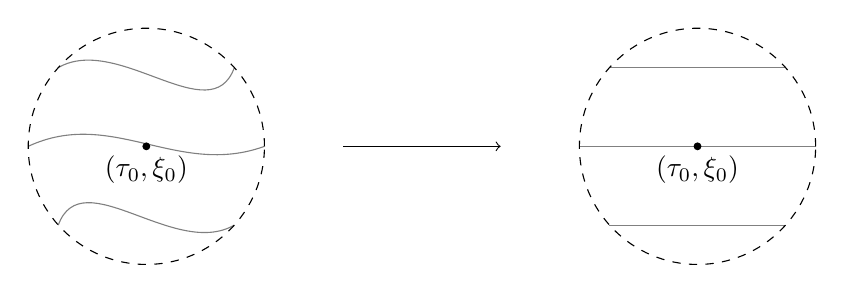
\begin{tikzpicture}
% Smooth curve lines passing over the circle on the left
              \draw[gray,smooth] (-1.118,1) to[out=30, in=250] (1.118,1);
              \draw[gray,smooth] (-1.5,0) to[out=25, in=200] (1.5,0);
              \draw[gray,smooth] (-1.118,-1) to[out=70, in=210] (1.118,-1);
% Circle on the left
              \draw[dashed] (0,0) circle (1.5cm);
              \fill (0,0) circle (0.05cm);
              \node[below] at (0,0) {$(\tau_0, \xi_0)$};
% Straight lines passing over the circle on the right
              \draw[gray] ({7 - sqrt(1.5 * 1.5 - 1)},1) -- ({7 + sqrt(1.5 * 1.5 - 1)},1);
              \draw[gray] (5.5,0) -- (8.5,0);
              \draw[gray] ({7 - sqrt(1.5 * 1.5 - 1)},-1) -- ({7 + sqrt(1.5 * 1.5 - 1)},-1);
% Circle on the right
              \draw[dashed] (7,0) circle (1.5cm);
              \fill (7,0) circle (0.05cm);
              \node[below] at (7,0) {$(\tau_0, \xi_0)$};
% Arrow connecting the two circles
              \draw[->] (2.5,0) -- (4.5,0);
        \end{tikzpicture}\]
    \provehere{
    Рассмотрим $I(\tau_0, \xi_0)$, и выберем $[a, b] \subset I(\tau_0, \xi_0)$ ($[a, b] \ni \tau_0$).
        Пусть $\eps > 0$, обозначим $R \coloneqq \defset{(t, x) \in [a, b] \times \R^n}{|x - x(t, \tau_0, \xi_0) \le \eps} \subset G$.

    По теореме об интегральной непрерывности $\exists \delta > 0: \forall \xi: |\xi - \xi_0| \le \delta \then (t, x(t, \tau_0, \xi)) \in R$ при $t \in [a, b]$.

    Положим $V = \defset{(t, x) \in [a, b] \times \R^n}{|x(t, \tau_0, \xi) - x(t, \tau_0, \xi_0) < \eps}$ --- это окрестность $(\tau_0, \xi_0)$.
        Построим $g: \overline{V} \map \R^{n + 1}$ следующим образом:
    \[g(t, \xi) = (t, x(t, \tau_0, \xi))\]
    $g$ непрерывна на $\overline{V}$:
    \[\abs{g(t, \xi) - g(t', \xi')} \le \underbrace{|x(t, \tau_0, \xi) - x(t', \tau_0, \xi)|}_{\abs{\int\limits_{t}^{t'}f(s, x(s, \tau_0, \xi))\d s} \le M|t - t'|} + \underbrace{|x(t', \tau_0, \xi) - x(t', \tau_0, \xi')|}_{\text{по теореме об интегральной непрерывности }\to 0}\]
    Инъективность $g$ прямо следует из теоремы единственности: $g(t, \xi) = g(t', \xi') \then t = t' \text { и } x(t, \tau_0, \xi) = x(t, \tau_0, \xi') \then \xi = \xi'$.

    Теперь построим обратное отображение $h$. Пусть $\overline{W} = g\left(\overline{V}\right)$, $U \coloneqq \Int\left(\overline{W}\right)$.
        Инъективное отображение компакта --- гомеоморфизм на образ, поэтому $\exists h: U \map V$ --- искомый гомеоморфизм.
    }
    }
    Пусть мы всё ещё рассматриваем систему $\dot{x} = f(t, x), x \in \R^n, f \in C, \Lip_{x,loc}(G)$.
    \theorem[О дифференциальном выпрямлении]{
        $\forall (\tau_0, \xi_0) \in G: \exists$ окрестность $U \ni (\tau_0, \xi_0)$, и $\exists$ диффеоморфизм $h: \overline{U} \map \R^{n + 1}$ (гомеоморфизм на образ $h$, такой, что $h, h^{-1}$ дифференцируемы), переводящий пересечение интегральных кривых с $\overline{U}$ в отрезки параллельных прямых.
    \provehere{
        Параллельно доказательству предыдущей теоремы построим $g$.
        То, что $g \in C^1$ следует из того, что решение дифференцируемо по $t$ и по начальным данным.

    Дальше мы хотим применить теорему об обратной функции, для этого надо показать невырожденность $\det \der{g}{(t, \xi)}\big|_{(\tau_0, \xi_0)}$.
    Расписав покомпонентно $g = (t, \xi)$, получаем \[\der{g}{(t, \xi)} = \vect{1 & 0 \\ \der{x}{t} & \der{x}{\xi}}\]
    Достаточно показать, что $\der{x}{\xi}$ невырождена, но это фундаментальная матрица системы в вариациях.

    Значит, по теореме об обратной функции $g$ --- диффеоморфизм окрестности $(\tau_0, \xi_0)$ на окрестность $(\tau_0, \xi_0)$.
    }
    }
    \section{Теорема Коши}
    \subsection{Кратные степенные ряды}
    \subsubsection{Многомерное суммирование}
    В случае обычных рядов $\sum\limits_{k = 0}^{\infty}a_k$ мы работаем с частичными суммами $\sum\limits_{k = 0}^{m}a_k$, которые куда-то стремятся.

    Случай многомерного индекса выглядит так: имеется набор чисел $a_{k_1, \dots, k_n}$, где $k_i \in \N_{0}$.

    Назовём суммой ряда $\sum\limits_{k_1 = \cdots = k_n = 0}^{\infty}a_{k_1, \cdots, k_n}$ сумму семейства $\defset{a_{k_1, \cdots, k_n}}{k_1, \cdots, k_n \in \N_{0}}$.

    Ещё это можно записать так: если $A$ --- сумма семейства, то по определению $\forall \eps > 0: \exists N: \forall m_1, \cdots, m_n \ge N: \abs{\sum\limits_{m_1, \cdots, m_n}a_{*} - A} < \eps$, где $\sum\limits^{m_1, \cdots, m_n}a_{*} \coloneqq \sum\limits_{k_1 = 0}^{m_1} \cdots \sum\limits_{k_n = 0}^{m_n}a_{k_1, \cdots, k_n}$ --- краткое обозначение для частичной суммы.

    Работая с абсолютно сходящимися многомерными рядами, мы сможем выполнять все действия над ними, какие захотим (например, потому что можно всё перевести на язык суммируемых семейств).
    \subsubsection{Многомерные степенные ряды}
    Кратные степенные ряды определяются исходя из обычных кратных рядов: пусть $x = \vect{x_1, \cdots, x_n}$, зафиксируем $x^0 = \vect{x_1^0, \cdots, x_n^0}$, и рассмотрим ряд
    \[\sum\limits_{k_1, \cdots, k_n}^{\infty}a_{k_1, \cdots, k_n}(x_1 - x_1^0)^{k_1} \proddots (x_n - x_n^0)^{k_n}\]
    \statement[Радиус сходимости]{
    Если ряд сходится для $(x_1^*, \cdots, x_n^*)$, то он сходится для любого $(x_1, \cdots, x_n): |x_i - x_i^0| < |x_i^* - x_i^0|$.
    }
    \statement[Мажоратные ряды]{
        Пусть есть ряд $\sum\limits_{k_1, \cdots, k_n}^{\infty}b_{k_1, \cdots, k_n}(x_1 - x_1^0)^{k_1}\proddots (x_n - x_n^0)^{k_n}$. Если все $\abs{a_{k_1, \cdots, k_n}} \le b_{k_1, \cdots, k_n}$, и ряд степенной ряд $b$ сходится, то и степенной ряд $a$ сходится.
    }
    \statement[Специальный ряд]{
    При $|x_i| < 1$ следующий ряд (многомерная геометрическая прогрессия) сходится: \[\sum\limits_{k_1, \cdots, k_n}^{\infty}x_1^{k_1}\proddots x_n^{k_n} = \frac{1}{(1 - x_1)\proddots (1 - x_n)}\]
    }

    \newlection{2 декабря 2023 г.}
    //todo
    \newlection{8 декабря 2023 г.}
    В прошлый раз была доказана теорема Коши: если $f$ --- аналитическая функция, то решение уравнения $\dot{x} = f(t, x)$ тоже аналитическое.

    \theorem[Коши, для линейных систем]{
    Рассмотрим задачу Коши с нулевыми начальными данными $(t_0, x_0) = (0, 0)$ в рамках системы $\dot{x} = p(t)x + q(t)$, где $x \in \R^n, p \in M_{n\times n}(\R),q \in \R^n$, причём коэффициенты аналитические: $p(t) = \sum\limits_{k = 0}^{\infty}p^{(k)}t^k, q(t) = \sum\limits_{k = 0}^{\infty}q^{(k)}t^k$, и они сходятся при $|t| < r_0$, здесь $r_0 > 0$.

        Тогда утверждается, что у решения $x$ имеется тот же радиус сходимости $r_0$.
    \provehere{
    Пусть решение представимо в виде $x = (x_1, \dots, x_n)$, $x_i = \sum\limits_{k = 1}^{\infty}a_k^{(i)}t^k$.

    Эти коэффициенты получены так: формально дифференцируя, получаем $\dot{x}_i = \sum\limits_{l = 1}^{\infty}la_l^{(i)}t^{l - 1}$, значит \[x_i = \sum\limits_{k = 1}^{\infty}a_k^{(i)}t^k = \sum\limits_{j = 1}^{n}\sum\limits_{k = 0}^{\infty}p_{i,j}^{(k)}t^k\underbrace{\left(\sum\limits_{l = 1}^{\infty}a_l^{(j)}t^l\right)}_{x_j} + \sum\limits_{k = 0}^{\infty}q_k^{(i)}t^k\]
    Приравнивая коэффициенты при равных степенях $t$, получаем \[\all{t^0:& a_1^{(i)} = q_0^{(i)} \\ t^1:&2a_2^{(i)} = \sum\limits_{j = 1}^{n}p_{i,j}^{(0)}a_1^{(i)} + q_{1}^{(i)} \\ &\ddots}\]
    В общем виде, это записывается так: $t^{m-1}: ma_m^{(i)} = P_m\left(p_{i,j}^{(k)}, a_l^{(j)}, q_i^{(m - 1)}\right)_{k \le m - 1, l \le m - 1}$, здесь $P_m$ --- некий многочлен с неотрицательными коэффициентами (они получены произведением и суммой членов).

    Теперь надо построить мажорирующую систему.
        Берём $r \in (0, r_0)$.
        Трюк Коши говорит, что если подставить такое $r$, то члены будут ограничены, то есть $\exists M \in \R: \abs{p_{i,j}^{(k)}r^k} \le M$, или же $\abs{p_{i,j}^{(k)}} \le \frac{M}{r^k}$. Аналогично $\abs{q_i^{(k)}} \le \frac{M}{r^k}$.

        В качестве мажорантной системы возьмём систему с искомыми функциями $z_1, \dots, z_n$, определёнными так: $\dot{z}_i = \sum\limits_{j = 1}^{n}\sum\limits_{k = 0}^{\infty}\frac{M}{r^k}t^k z_j + \sum\limits_{k = 0}^{\infty}\frac{M}{r^k}t^k$.
    Эти геометрические прогрессии можно просуммировать: \[\dot{z}_i = \sum\limits_{j = 0}^{n}\frac{M}{1 - \frac{t}{r}}z_j + \frac{M}{1 - \frac{t}{r}}\]
    Мажорирующая система линейна, её решение можно получить так: пусть $z_1 = \dots = z_n = u$, тогда $\dot{u} = \frac{M}{1 - \frac{t}{r}}(nu + 1)$.
    Это линейное уравнение первого порядка, коэффициенты аналитичны при $|t| < r$.
        В прошлой лекции была получена формула, в которой коэффициенты --- тоже аналитические функции при $|t| < r$.

    Получив оценку на сходимость мажорирующей системы, мы уже всё доказали.
    }
    }
    \chapter{Автономные системы}
    \emph{Автономные системы} --- системы, у которых правая часть не зависит от $t$.

    А именно, рассматривается система $\dot{x} = f(x)$, где предполагается, что $f \in \Lip_{x,loc}(H), H \subset \R_x^n$ --- область.
    Так как $f$ локально липшицева по аргументу, то она непрерывна.
    Пространство, где ищутся решения --- $\R^n_x$ --- \emph{фазовое пространство}.

    Можно применить общую теорию к области $G = \R \times H \subset \R_{t,x}^{n + 1}$, получается, $H$ --- область существования и единственности.
    \theorem{
    Если $x(t)$ --- решение на $(a, b)$, то $\forall c \in \R$: сдвиг решения $x(t + c)$ --- решение на $(a - c, b - c)$.
    }
    \definition[Траектория]{
    Проекция интегральной кривой на фазовое пространство.
    }
    Траектория не зависит от сдвига, и, вообще говоря (кроме вырожденных случаев), это --- гладкая кривая, по которой можно понять и направление движения решения.

    Пусть $x_0 \in H$, выберем главным решением $\phi(t, x_0) \coloneqq x(t, 0, x_0)$ --- решение задачи Коши с начальным данным $x(0) = x_0$.
    По определению $\phi(0, x_0) = x_0$.
    Максимальный промежуток решения $\phi(t, x_0)$ будет обозначаться за $I(x_0)$.
    \theorem[Групповое свойство автономных систем]{
    Если $s, t, t + s \in I(x_0)$, то $\phi(t + s, x_0) = \phi(t, \phi(s, x_0))$.
    \provehere{
    Рассмотрим обе части, как функции от $t$.
        Левая часть --- сдвиг какого-то решения, правая часть --- какое-то решение, и при $t = 0$ части равны друг другу.
    }
    }
    \section{Виды траекторий}
    \subsection{Точка покоя}
    \definition[Точка покоя]{
    Такая точка $x_0$, что $\phi(t, x_0) \equiv x_0$ --- решение.
    }
    Несложно видеть, что точки покоя автономной системы --- это $\defset{x_0 \in H}{f(x_0) = 0}$.
    \subsection{Замкнутая траектория}
    Пусть $x_0$ --- не точка покоя, причём нашлись $t_1 < t_2: \phi(t_1, x_0) = \phi(t_2, x_0)$.
    Можно считать, что при $t \in (t_1, t_2): \phi(t, x_0) \ne \phi(t_1, x_0)$.
    Это в частности следует из того, что если $x_0$ --- не точка покоя, то любая точка траектории --- не точка покоя.

    Обозначим $\omega \coloneqq t_2 - t_1$.
    \fact{$\phi(t, x_0)$ --- $\omega$-периодическая функция (по $t$).
    \provehere{
        Рассмотрим $\psi(t) = \phi(t + \omega, x_0)$.
        Это решение, как сдвиг. Оно определено хотя бы на отрезке $[t_1 - \omega, t_2 - \omega]$.
    \[\psi(t_1) = \phi(t_1 + \omega, x_0) = \phi(t_2, x_0) = \phi(t_1, x_0)\]
    Значит, по единственности $\psi(t) \equiv \phi(t, x_0)$.
    }}
    \definition[Замкнутая траектория]{
    Траектория периодического решения.
    }
    Понятно, что замкнутая траектория --- замкнутая несамопересекающаяся регулярная (касательный вектор не нулевой) кривая в фазовом пространстве.
    \subsection{Обыкновенная траектория}
    Пусть $\forall t_1, t_2 \in I(x_0): \phi(t_1, x_0) \ne \phi(t_2, x_0)$ при $t_1 \ne t_2$.

    В таком случае траектория --- просто непрерывный образ $I(x_0)$.
    \ok
    \example{
    Рассмотрим систему $\dot{x} = 1 + x^2$. Тогда $\phi(t, 0) = \tg t$, $I(0) = \left(-\frac{\pi}{2}, \frac{\pi}2\right)$, траектория --- вся ось $\R$.
    Однако эта траектория --- образ ограниченного интервала, что может быть неудобно. Поборемся несколько искусственным способом с этим ниже.
    }
    Пусть $f$ определена на всём пространстве $\R^n_x$.

    Рассмотрим вместе с системой $\dot{x} = f(x)$ другую систему $\dot{y} = g(y)$, где $g(y) = \frac{f(y)}{1 + \|f(y)\|^2_{\text{euclid}}}$.
    У новой системы $|g(y)| < 1$, и из теоремы об уравнениях, сравнимых с линейными~(\cref{compared}), любое решение $y$ продолжимо на всю ось $\R$.

    Пусть $y(t)$ --- решение системы $\dot{y} = g(y)$ c начальным условием $y(0) = x_0$.
    Рассмотрим $h: \R \map \R, h(\tau) = \int\limits_{0}^{\tau}\frac{\d s}{1 + \|f(y(s))\|^2_{\text{euclid}}}$. $h$ --- непрерывная функция, $\dot{h} > 0$.
    Пусть $\Image h = I$.

    Значит, имеется обратная функция $\theta = h^{-1}: I \map \R$.
    Тогда $\theta(h(\tau)) = \tau$, и, дифференцируя это равенство, получаем $\frac{\d \theta}{\d t}(h(\tau)) \cdot \frac{\d h}{\d \tau} = 1$.
    То есть
    \[\frac{\d\theta}{\d t}(t) = \frac{\d \theta}{\d t}(h(\tau)) = 1 + \|f(y(\tau))\|^2_{\text{euclid}} = 1 + \|f(y(\theta(t)))\|^2_{\text{euclid}}\]
    Утверждается, что $z(t) = y(\theta(t))$ --- решение первой системы $\dot{z} = f(z)$.
    В самом деле,
    \[\frac{\d z}{\d t} = \frac{\d y}{\d \theta}(\theta(t)) \cdot \frac{\d \theta}{\d t} = \frac{f(\theta(t))}{1 + \|f(y(\theta(t)))\|^2_{\text{euclid}}}(1 + \|f(y(\theta(t)))\|^2_{\text{euclid}}) = f(z(t))\]

    Таким образом получается, что решению $y: \R \map \R^n$ системы $\dot{y} = f(y)$ с начальным данным $y(0) = x_0$ соответствует некоторое решение $z: I \map \R^n$ системы $\dot{z} = f(z)$ с тем же начальным данным $z(0) = x_0$, причём их траектории одинаковы.

    Значит, если мы хотим исследовать возможные траектории автономных уравнений, нам достаточно исследовать траектории решений, определённых на всей оси.
    \section{Классификация Пуанкаре}
    Пуанкаре задавался вопросом о траекториях: все ли траектории примыкают к началу координат, и есть ли предельное положение касательных.

    В случае положительного ответа на оба вопроса траектории называются \emph{узел}, и в зависимости от количества предельных положений касательных, он называется \emph{обыкновенный} ($2$), \emph{дикритический} ($\infty$), вырожденный ($1$).

    Если же часть касательных примыкает к нулю, а часть нет, то это --- \emph{седло}.

    Далее ниже приводится классификация всевозможных траекторий уравнения $\dot{z} = Bz$, где $z \in \R^2$, $B \in GL(2, \R)$.

    Введём новую переменную $u$, связанную со старой равенством $z = Su$, где $S \in GL(2, \R)$ --- неособая замена координат плоскости.
    Уравнение преобразуется к виду $\dot{u} = S^{-1}BS u$, и, конечно, хочется, чтобы $A \coloneqq S^{-1}BS$ было жордановой формой матрицы $B$.

    Перейдём к привычным координатам $u = \vect{x \\ y}$, и рассмотрим разные возможные виды $A$.
    \bullets{
    \item $\lambda, \mu \in \R$ --- собственные числа $A$, причём $\lambda \ne \mu$.
    Тогда уравнение сводится к
    \[\all{\dot{x} = \lambda x \\ \dot{y} = \lambda y}\]
    У системы есть симметрии: решению $(x(t), y(t))$ соответствуют другие решения $(-x, y), (x, -y), (-x, -y)$.

    Имеется точка покоя $(0, 0)$. Далее, открытые полуоси тоже являются траекториями решений $(x_0 e^{\lambda t}, 0)$ и $(0, y_0 e^{\mu t})$.

    Теперь изобразим траекторию, лежащую внутри первой четверти. $x(t) = x_0 e^{\lambda t}, y(t) = y_0 e^{\mu t}$, и несложные преобразования дают $t = \frac{1}{\lambda}\log\left(\frac{x}{x_0}\right)$ и $y = C x^{\frac{\mu}{\lambda}}$.
    \bullets{
    \item Если $\mu$, $\lambda$ одного знака, то будут выпуклые или вогнутые возрастающие из нуля координат функции.
    Такое расположение траекторий называется \emph{обыкновенный узел}.
        \[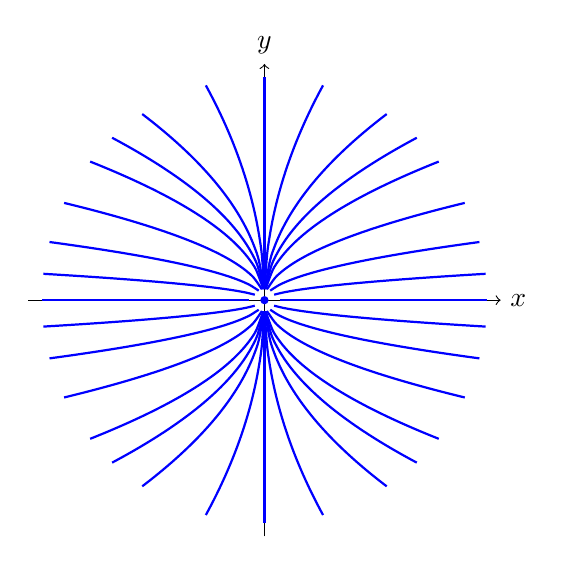
\begin{tikzpicture}
              \draw[->] (-3,0) -- (3,0) node[right] {$x$};
              \draw[->] (0,-3) -- (0,3) node[above] {$y$};
              \pgfmathsetmacro\r{0.01};
              \pgfmathsetmacro\R{4};
              \foreach \c in {0.02,0.1,0.3,0.7,1.1,1.8,5} {
                  \draw[scale=1,domain={-\c+sqrt(\c*\c+2*\r)}:{-\c+sqrt(\c*\c+2*\R)},smooth,variable=\x,blue,line width=0.8pt] plot ({\x},{sqrt(2*\c*\x)});
                  \draw[scale=1,domain={-\c+sqrt(\c*\c+2*\r)}:{-\c+sqrt(\c*\c+2*\R)},smooth,variable=\x,blue,line width=0.8pt] plot ({\x},{-sqrt(2*\c*\x)});
                  \draw[scale=1,domain={-\c+sqrt(\c*\c+2*\r)}:{-\c+sqrt(\c*\c+2*\R)},smooth,variable=\x,blue,line width=0.8pt] plot ({-\x},{sqrt(2*\c*\x)});
                  \draw[scale=1,domain={-\c+sqrt(\c*\c+2*\r)}:{-\c+sqrt(\c*\c+2*\R)},smooth,variable=\x,blue,line width=0.8pt] plot ({-\x},{-sqrt(2*\c*\x)});
              }
              \foreach \x/\y in {1/0,0/1,-1/0,0/-1} {
                  \pgfmathsetmacro{\l}{sqrt(2 * \R)}
                  \draw[blue,line width=0.8pt] (0.2*\x,0.2*\y) -- (\l*\x,\l*\y);
              }
              \fill[blue] (0,0) circle (1.5pt);
        \end{tikzpicture}
        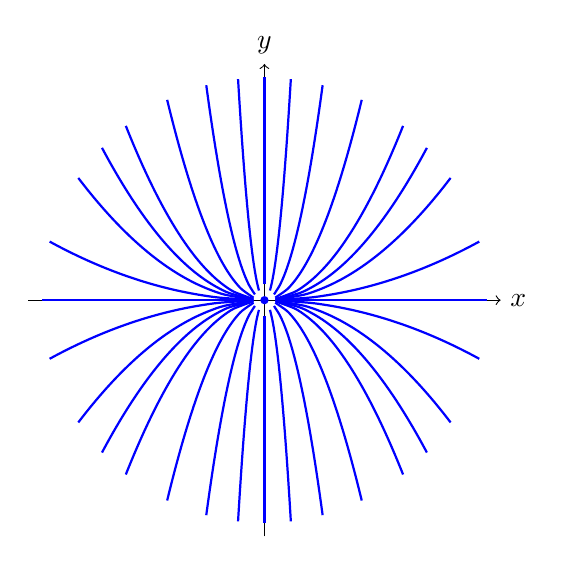
\begin{tikzpicture}
             \draw[->] (-3,0) -- (3,0) node[right] {$x$};
             \draw[->] (0,-3) -- (0,3) node[above] {$y$};
             \pgfmathsetmacro\r{0.01};
             \pgfmathsetmacro\R{4};
             \foreach \c in {0.02,0.1,0.3,0.7,1.1,1.8,5} {
                 \draw[scale=1,domain={-\c+sqrt(\c*\c+2*\r)}:{-\c+sqrt(\c*\c+2*\R)},smooth,variable=\x,blue,line width=0.8pt] plot ({sqrt(2*\c*\x)},{\x});
                 \draw[scale=1,domain={-\c+sqrt(\c*\c+2*\r)}:{-\c+sqrt(\c*\c+2*\R)},smooth,variable=\x,blue,line width=0.8pt] plot ({-sqrt(2*\c*\x)},{\x});
                 \draw[scale=1,domain={-\c+sqrt(\c*\c+2*\r)}:{-\c+sqrt(\c*\c+2*\R)},smooth,variable=\x,blue,line width=0.8pt] plot ({sqrt(2*\c*\x)},{-\x});
                 \draw[scale=1,domain={-\c+sqrt(\c*\c+2*\r)}:{-\c+sqrt(\c*\c+2*\R)},smooth,variable=\x,blue,line width=0.8pt] plot ({-sqrt(2*\c*\x)},{-\x});
             }
             \foreach \x/\y in {1/0,0/1,-1/0,0/-1} {
                 \pgfmathsetmacro{\l}{sqrt(2 * \R)}
                 \draw[blue,line width=0.8pt] (0.2*\x,0.2*\y) -- (\l*\x,\l*\y);
             }
             \fill[blue] (0,0) circle (1.5pt);
        \end{tikzpicture}\]
        \item Если $\mu$, $\lambda$ разных знаков, то будут своеобразные гиперболы.
        В сечении гиперболического параболоида получатся такие кривые, поэтому семейство траекторий называется \emph{седло}.
        \[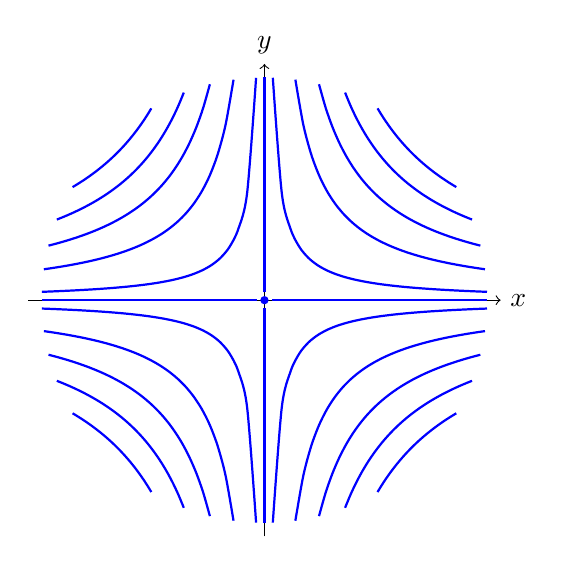
\begin{tikzpicture}
            \draw[->] (-3,0) -- (3,0) node[right] {$x$};
            \draw[->] (0,-3) -- (0,3) node[above] {$y$};
            \pgfmathsetmacro\r{4};
            \foreach \c in {-3.5,-2.7,...,0.5,0.3,1.1,...,4.3} {
                \draw[domain={sqrt(\r-sqrt(\r*\r-\c*\c))}:{sqrt(\r+sqrt(\r*\r-\c*\c))},smooth,variable=\x,blue,line width=0.8pt] plot ({\x},{\c/\x});
                \draw[domain={-sqrt(\r+sqrt(\r*\r-\c*\c))}:{-sqrt(\r-sqrt(\r*\r-\c*\c))},smooth,variable=\x,blue,line width=0.8pt] plot ({\x},{\c/\x});
            }
            \foreach \x/\y in {1/0,0/1,-1/0,0/-1} {
                \pgfmathsetmacro{\l}{sqrt(2 * \r)}
                \draw[blue,line width=0.8pt] (0.1*\x,0.1*\y) -- (\l*\x,\l*\y);
            }
            \fill[blue] (0,0) circle (1.5pt);
        \end{tikzpicture}\]
    }
    \newlection{15 декабря 2023 г.}
    \item Теперь пусть $\lambda, \mu \in \R$ --- собственные числа $A$, причём $\lambda = \mu$.
    Здесь жорданова форма может иметь два разных вида.
    \bullets{
    \item Пусть $A = \vect{\lambda & 0 \\ 0 & \lambda}$.
        Тогда все траектории --- всевозможные лучи, исходящие из нуля координат.
    Такое расположение Пуанкаре назвал \emph{дикритический узел}.
        \[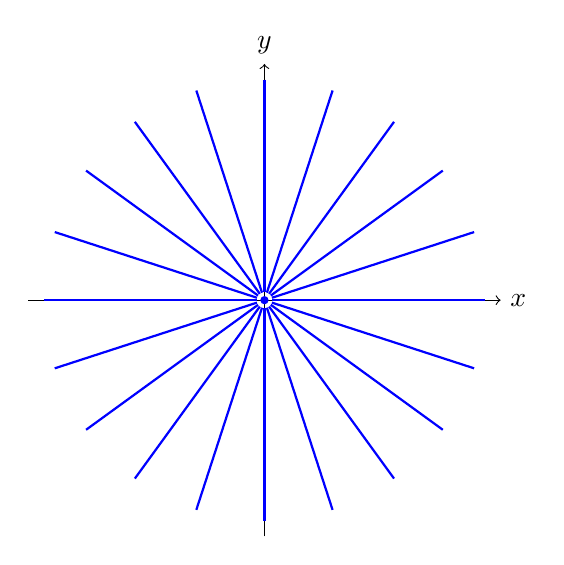
\begin{tikzpicture}
              \draw[->] (-3,0) -- (3,0) node[right] {$x$};
              \draw[->] (0,-3) -- (0,3) node[above] {$y$};
              \pgfmathsetmacro\r{2.8};
              \pgfmathsetmacro\R{0.1};
              \foreach \alpha in {0,18,...,360} {
                  \draw[blue,line width=0.8pt] ({\r*cos(\alpha)},{\r*sin(\alpha)}) -- ({\R*cos(\alpha)},{\R*sin(\alpha)});
              }
              \fill[blue] (0,0) circle (1.5pt);
        \end{tikzpicture}\]
    \item Пусть $A = \vect{\lambda & 0 \\ 1 & \lambda}$. Тогда решение системы $\all{\dot{x}, \lambda x \\ \dot{y} = x + \lambda y}$.
    Здесь симметрий меньше --- есть только центральная $(x, y) \leftrightsquigarrow (-x, -y)$, но нет осевых.
    \bullets{
    \item Имеется траектория $\all{x = 0 \\ y = y_0 e^{\lambda t}}$, делящая плоскость на две половинки, и картинку можно рисовать только в правой полуплоскости, а потом отражать.
    \item Пусть $x = x_0 e^{\lambda t}$. Тогда на $y$ получается линейное уравнение $\dot{y} = \lambda y + x_0 e^{\lambda t}$.
        Решая его, получаем $y = (x_0 t + C)e^{\lambda t}$
    \item Выражая $t = \frac{1}{\lambda}\log\left(\frac{x}{x_0} + C\right)$, получаем уравнение кривых $y = x\left(\frac{1}{\lambda}\log(x) + \tilde{C}\right)$.
    $y(x) \underset{x \to 0}\Map 0$, зато $y'(x) \underset{x \to 0}\Map \infty$, и знак бесконечности противоположен знаку $\lambda$.

    Эта траектория называется \emph{вырожденный узел}.
        \[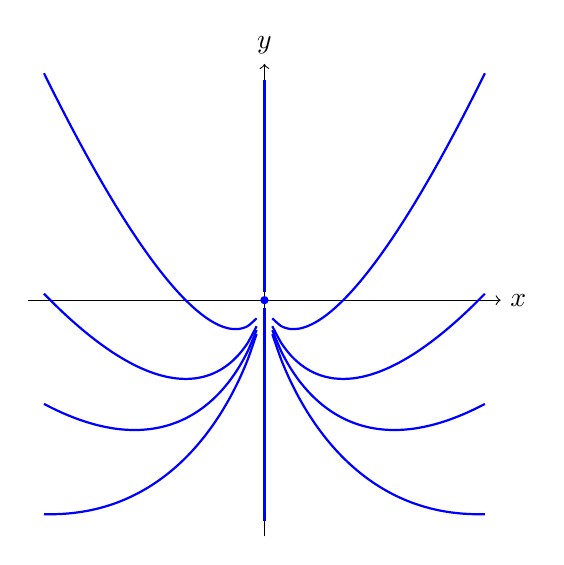
\begin{tikzpicture}
              \draw[->] (-3,0) -- (3,0) node[right] {$x$};
              \draw[->] (0,-3) -- (0,3) node[above] {$y$};
              \pgfmathsetmacro\r{2.8};
              \pgfmathsetmacro\R{0.1};
              \foreach \c in {-2,-1.5,-1,0} {
                  \draw[scale=1,domain=0.1:2.8,smooth,variable=\x,blue,line width=0.8pt] plot ({\x},{\x*(ln(\x)+\c)});
                  \draw[scale=1,domain=0.1:2.8,smooth,variable=\x,blue,line width=0.8pt] plot ({-\x},{\x*(ln(\x)+\c)});
              }
              \foreach \x/\y in {0/1,0/-1} {
                  \draw[blue,line width=0.8pt] (0.1*\x,0.1*\y) -- (\r*\x,\r*\y);
              }
              \fill[blue] (0,0) circle (1.5pt);
        \end{tikzpicture}\]
    }
    }
    \item Теперь пусть собственные числа $B$ комплексные: $\lambda_{1,2} = a \pm bi$.
    Тогда можно сопряжением привести $B$ к виду $A \coloneqq S^{-1}BS = \vect{a & -b \\ b & a}$.

    Тогда система имеет вид $\all{\dot{x} = ax - yb \\ \dot{y} = bx + ay}$.
        Переходя к полярным координатам, получаем $\all{\dot{r}\cos \phi - r \sin \phi \cdot \dot{\phi} = ar \cos \phi - br \sin \phi \\ \dot{r}\sin\phi + r\cos\phi \cdot \dot{\phi} = br \cos \phi + ar \sin \phi}$.
    Выражая отдельно $\dot{r}$ и $\dot{\phi}$, получаем $\all{\dot{r} = ar \\ r \dot{\phi} = br}$.

    Теперь данную систему несложно решить $\all{r(t) = r_0 e^{a t} \\ \phi(t) = bt + \phi_0}$, и выразить, например, как функцию $r(\phi) = r_0 e^{\frac{a}{b}(\phi - \phi_0)}$, или $r = \tilde{r}_0e^{\frac{a}{b}\phi}$.
    \bullets{
    \item При $a = 0$ экспоненты чисто мнимая, и траектории --- концентрические окружности с центром в нуле.
    Здесь кроме точки покоя никакая к нулю не примыкают, Пуанкаре дал название \emph{центр} этому виду траекторий.
    \item Наконец, если $a \ne 0$, то получаются логарифмические спирали, образующие \emph{фокус} --- все траектории примыкают к нулю, но ни одна не имеет предельного положения касательной.
        \[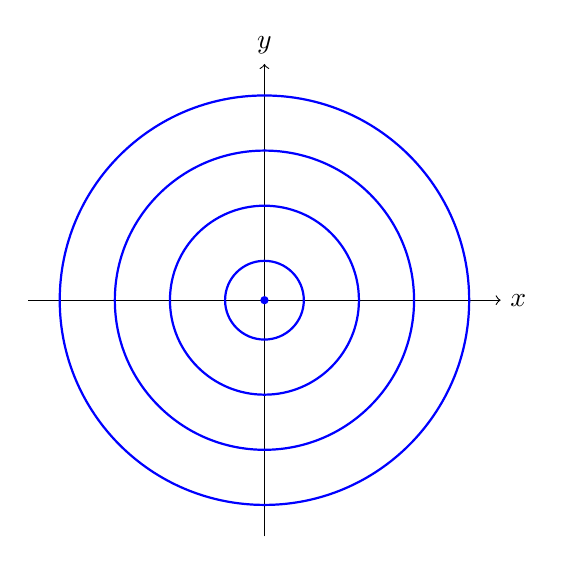
\begin{tikzpicture}
              \draw[->] (-3,0) -- (3,0) node[right] {$x$};
              \draw[->] (0,-3) -- (0,3) node[above] {$y$};
              \foreach \r in {0.5,1.2,...,2.6} {
                  \draw[blue,line width=0.8pt] (0,0) circle ({\r});
              }
              \fill[blue] (0,0) circle (1.5pt);
        \end{tikzpicture}
        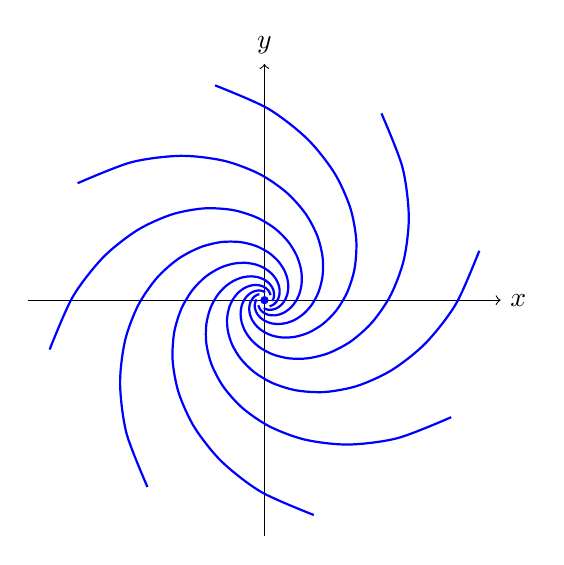
\begin{tikzpicture}
             \draw[->] (-3,0) -- (3,0) node[right] {$x$};
             \draw[->] (0,-3) -- (0,3) node[above] {$y$};
             \foreach \alpha in {0,45,...,315} {
                 \draw[scale=1,domain={ln(0.1)}:{ln(2.8)},smooth,variable=\x,blue,line width=0.8pt] plot ({exp(\x)*cos(\alpha+100*\x)},{exp(\x)*sin(\alpha+100*\x)});
             }
             \fill[blue] (0,0) circle (1.5pt);
        \end{tikzpicture}\]
    }
    }
В дополнение к данной классификации мы приведём упрощённую формулировку теоремы, которая рассматривает нелинейные системы.
    \intfact[Теорема Пуанкаре]{
        Рассматривается уравнение $\dot{z} = Bz + F(z)$, где $B \in GL(2, \R)$, $F(0) = 0, \der{F}{z}(0) = \0$, причём в некоторой окрестности нуля $U: F \in C^2(U)$.

    Если собственные числа $B$ не чисто мнимые, то существует диффеоморфизм $h$, переводящий окрестность нуля в окрестность нуля, такой, что $h \in C^1, h(0) = 0, \der{h}{z}(0) = E$, и $h$ отображает траектории $\dot{z} = Bz$ на траектории $\dot{z} = Bz + F(z)$.
    }
    Иными словами, если траектории $\dot{z} = Bz$ образуют не центр, то локально в нуле расположение решений линейных и нелинейных систем схожи.

    \note[Проблема центра и фокуса]{
    Даже для полиномиальных систем и на сей день не найдены необходимые и достаточные условия, при которых малое возмущение центр оставляет центром.
    }
\end{document}



